\documentclass[notes,11pt, aspectratio=169]{beamer}

\usepackage{pgfpages}
% These slides also contain speaker notes. You can print just the slides,
% just the notes, or both, depending on the setting below. Comment out the want
% you want.
\setbeameroption{hide notes} % Only slide
%\setbeameroption{show only notes} % Only notes
% \setbeameroption{show notes on second screen=right} % Both

\usepackage{helvet}
% \usepackage[default]{lato}
\usepackage{array}
\usepackage[longnamesfirst]{natbib}
% \bibliographystyle{plain}
% \usepackage{apalike}
\bibliographystyle{apalike}
% \addbibresource{../manuscript/references.bib}
% \usepackage[natbib, maxcitenames=3, mincitenames=11, style=apa]{biblatex}

\usepackage{tikz}
\newcommand*\circled[4]{\tikz[baseline=(char.base)]{
 \node[shape=circle, fill=#2, draw=#3, text=#4, inner sep=2pt] (char) {#1};}}
\usepackage{verbatim}
\setbeamertemplate{note page}{\pagecolor{yellow!5}\insertnote}
\usetikzlibrary{positioning}
\usetikzlibrary{snakes}
\usetikzlibrary{calc}
\usetikzlibrary{arrows}
\usetikzlibrary{decorations.markings}
\usetikzlibrary{shapes.misc}
\usetikzlibrary{matrix,shapes,arrows,fit,tikzmark}
\usepackage{amsmath}
\usepackage{mathpazo}
\usepackage{hyperref}
\usepackage{lipsum}
\usepackage{multimedia}
\usepackage{graphicx}
\usepackage{multirow}
\usepackage{graphicx}
\usepackage{dcolumn}
\usepackage{bbm}
\usepackage{adjustbox} % Shrink stuff
\usepackage{cancel}
\newcolumntype{d}[0]{D{.}{.}{5}}

\usepackage{changepage}
\usepackage{appendixnumberbeamer}
\newcommand{\beginbackup}{
 \newcounter{framenumbervorappendix}
 \setcounter{framenumbervorappendix}{\value{framenumber}}
 \setbeamertemplate{footline}
 {
 \leavevmode%
 \hline
 box{%
 \begin{beamercolorbox}[wd=\paperwidth,ht=2.25ex,dp=1ex,right]{footlinecolor}%
% \insertframenumber \hspace*{2ex} 
 \end{beamercolorbox}}%
 \vskip0pt%
 }
 }
\newcommand{\backupend}{
 \addtocounter{framenumbervorappendix}{-\value{framenumber}}
 \addtocounter{framenumber}{\value{framenumbervorappendix}} 
}

% Fancy fit image command with an optional caption
\makeatletter
\newcommand{\fitimage}[2][\@nil]{
 \begin{figure}
 \begin{adjustbox}{width=0.9\textwidth, totalheight=\textheight-2\baselineskip-2\baselineskip,keepaspectratio}
 \includegraphics{#2}
 \end{adjustbox}
 \def\tmp{#1}%
 \ifx\tmp\@nnil
 \else
 \caption{#1}
 \fi
 \end{figure}
}
\makeatother

\usepackage{graphicx}
\usepackage[space]{grffile}
\usepackage{booktabs}

% These are my colors -- there are many like them, but these are mine.
\definecolor{blue}{RGB}{0,114,178}
\definecolor{red}{RGB}{213,94,0}
\definecolor{yellow}{RGB}{240,228,66}
\definecolor{green}{RGB}{0,158,115}

% % Environments
% \newtheorem{defin}{Definition.}
% \newtheorem{teo}{Theorem. }
% \newtheorem{lema}{Lemma. }
% \newtheorem{coro}{C
% \begin{frame}{Modeling Choice}orolary. }
% \newtheorem{prop}{Proposition. }
% \theoremstyle{definition}
% \newtheorem{examp}{Example. }
% % \numberwithin{problem}{subsection} 

\hypersetup{
 colorlinks=false,
 linkbordercolor = {white},
 linkcolor = {blue}
}


%% I use a beige off-white for my background
\definecolor{MyBackground}{RGB}{255,253,218}

%% Uncomment this if you want to change the background color to something else
%\setbeamercolor{background canvas}{bg=MyBackground}

%% Change the bg color to adjust your transition slide background color!
\newenvironment{transitionframe}{
 \setbeamercolor{background canvas}{bg=yellow}
 \begin{frame}}{
 \end{frame}
}

\setbeamercolor{frametitle}{fg=blue}
\setbeamercolor{title}{fg=black}
\setbeamertemplate{footline}[frame number]
\setbeamertemplate{navigation symbols}{} 
\setbeamertemplate{itemize items}{-}
\setbeamercolor{itemize item}{fg=blue}
\setbeamercolor{itemize subitem}{fg=blue}
\setbeamercolor{enumerate item}{fg=blue}
\setbeamercolor{enumerate subitem}{fg=blue}
\setbeamercolor{button}{bg=MyBackground,fg=blue,}
\setbeamercolor{theotem}{fg=blue} 

% If you like road maps, rather than having clutter at the top, have a roadmap show up at the end of each section 
% (and after your introduction)
% Uncomment this is if you want the roadmap!
% \AtBeginSection[]
% {
% \begin{frame}
% \frametitle{Roadmap of Talk}
% \tableofcontents[currentsection]
% \end{frame}
% }


\setbeamercolor{section in toc}{fg=blue}
\setbeamercolor{subsection in toc}{fg=red}
\setbeamersize{text margin left=1em,text margin right=1em} 

\newenvironment{wideitemize}{\itemize\addtolength{\itemsep}{10pt}}{\enditemize}

\usepackage{environ}
\NewEnviron{videoframe}[1]{
 \begin{frame}
 \vspace{-8pt}
 \begin{columns}[onlytextwidth, T] % align columns
 \begin{column}{.58\textwidth}
 \begin{minipage}[t][\textheight][t]
 {\dimexpr\textwidth}
 \vspace{8pt}
 \hspace{4pt} {\Large \sc \textcolor{blue}{#1}}
 \vspace{8pt}
 
 \BODY
 \end{minipage}
 \end{column}%
 \hfill%
 \begin{column}{.42\textwidth}
 \colorbox{green!20}{\begin{minipage}[t][1.2\textheight][t]
 {\dimexpr\textwidth}
 Face goes here
 \end{minipage}}
 \end{column}%
 \end{columns}
 \end{frame}
}

\title[]{\textcolor{blue}{Industry Heterogeneity and Wage Inequality}}
\author[MVB]{}
\institute[UW-Madison]{Mitchell Valdes-Bobes}

\date{\today}


\begin{document}
%%% TIKZ STUFF
\tikzset{ 
 every picture/.style={remember picture,baseline},
 every node/.style={anchor=base,align=center,outer sep=1.5pt},
 every path/.style={thick},
 }
\newcommand\marktopleft[1]{%
 \tikz[overlay,remember picture] 
 \node (marker-#1-a) at (-.3em,.3em) {};%
}
\newcommand\markbottomright[2]{%
 \tikz[overlay,remember picture] 
 \node (marker-#1-b) at (0em,0em) {};%
}
\tikzstyle{every picture}+=[remember picture] 
\tikzstyle{mybox} =[draw=black, very thick, rectangle, inner sep=10pt, inner ysep=20pt]
\tikzstyle{fancytitle} =[draw=black,fill=red, text=white]
%%%% END TIKZ STUFF

% % Title Slide
\begin{frame}
 \maketitle
\end{frame}
% % Outline Slide
% \begin{frame}
% \frametitle{Roadmap of Talk}
% \tableofcontents
% \end{frame}

% INTRO
% \begin{transitionframe}
% \begin{center}
% { \Huge \textcolor{black}{Introduction and Motivation}}
% \end{center}
% \end{transitionframe}
% \section{Motivation}
% \begin{frame}{What this talk is about?}
% \begin{wideitemize}
% \item I want to explore how the differences in industries' workforce composition impact the increasing wage disparities between workers.
% \end{wideitemize}
% \end{frame}
% Motivation Slide
\section{Introductuion and Motivation}
\begin{frame}{Introduction}
\begin{wideitemize}
 \item Wage Inequality has risen since the 1980s.
 \item The distribution of wages inside firms does not follow the same trend as the entire economy.
 \item \textcolor{blue}{Song, Price, Guvenen, Bloom, and Von Wachter (2019)}, show that a substantial part of the rise in dispersion has occurred between firms instead of within firms.
 % \begin{wideitemize}
 % \item \textbf{ Sorting effect:} high-wage workers are increasingly likely to work for more productive firms.
 % \item \textbf{ Segregation effect:} high-paying workers to be working with each other more frequently.
 % \end{wideitemize}
 \item At the same time there has been an increase in occupational and educational, segregation of employees.
\end{wideitemize}
\end{frame}

\begin{frame}{Introduction}
\begin{wideitemize}
 \item I want to focus on the relationship between the composition of the workforce (Labor Input Ratio)
 \begin{itemize}
 \item Skilled workers vs Unskilled workers
 \end{itemize}
 \item and wage inequality between those groups (the Skill Premium).
 \item I will use the model proposed by \textcolor{blue}{Krusell, Ohanian, Ríos‐Rull, and Violante (2000)} (KORV) to isolate two effects influencing the growth of the skill premium:
 \only<2-3>{
 \begin{wideitemize}
 \item the effect of the relative input of skilled vs. unskilled workers.
 \item the effect of skill-biased technological change. (Capital-skill complementarity hypothesis)
 \end{wideitemize}
 }
 \only<3>{
 \item I will analyze these effects have evolved industry level. 
 }
\end{wideitemize}
\end{frame}

\begin{frame}{Objectives}
This work has two primary objectives:
\vspace*{0.4cm}
\begin{wideitemize}
 \item Extend the analysis from KORV beyond the original period.
 \item Evaluate the capital-skill complementarity hypothesis at the industry level.
\end{wideitemize}
\vspace*{1cm}
\end{frame}


\begin{frame}{Motivation}
\begin{wideitemize}
 \item In a recent work \textcolor{blue}{Haltiwanger, Hyatt and Spletzer (2022)}, shows that the rise in wage inequality is concentrated in a small number of industries (about $10\%$).
 \begin{wideitemize}
 \item This work analyzes industries at the 4-digit NAICS level.
 \item I work with more aggregated data.
 \end{wideitemize}
 \item There is a fact that holds at a higher level:
 \begin{wideitemize}
 \item High-wage industries are more likely to exhibit larger skill-premium.
 \end{wideitemize}
\end{wideitemize}
\end{frame}

\section*{Data}

\begin{frame}{Industry Level Trends}
 \begin{center}
 \fitimage[Relationship between skill premium and mean wage.]{../images/correlations_wage_SP_slides.pdf}
 \end{center}
\end{frame}

% \begin{frame}{Model}
% \begin{wideitemize}
% \item I will use the model by~\cite{krusell2000capital} (henceforth \textbf{KORV}).
% \item Allows me to decompose the change of the wage premium paid to skilled workers into two effects:
% \begin{itemize}
% \item The effect of the relative supply of skilled to unskilled labor.
% \item The capital-skill complementary effect.
% \end{itemize}
% \end{wideitemize}
% \end{frame}

% \begin{frame}{LITERATURE}
% My work is related to...
% \begin{wideitemize}
% \item I will use the model by~\cite{krusell2000capital} (henceforth \textbf{KORV}).
% \item Allows me to decompose the change of the wage premium paid to skilled workers into two effects:
% \begin{itemize}
% \item The effect of the relative supply of skilled to unskilled labor.
% \item The capital-skill complementary effect.
% \end{itemize}
% \end{wideitemize}
% \end{frame}

\section*{Data}
\begin{frame}{Data}
 \begin{wideitemize}
 \item I constructed data series for wages, labor input, and capital input from 1963 to 2018.
 \begin{itemize}
 \item The original data from KORV covers the period from 1963 to 1992.
 \end{itemize}
 \item I followed the methodology of \textcolor{blue}{Ohanian, Orak and Shen (2021)}. 
 \item Re-create the same series for $56$ industry groups for the period from $1998$ to $2018$.
 \end{wideitemize}
 \end{frame}
 
\begin{frame}
\frametitle{Capital Data}
\begin{wideitemize}
 \item I obtained investment series in equipment $(I_e)$ and structures $(I_s)$ from NIPA.
 \item Equipment $(K_e)$ and structure $(K_s)$ capital series were constructed using the perpetual inventory method:
 \begin{equation*}\label{eq:capital_law_motion}
 K_{i_{t+1}} = (1 - \delta_{i_t}) K_{i_{t}} + I_{i_{t}} \qquad i\in\{e, s\}
 \end{equation*}
 \item For capital data at the industry level I used the BEA Fixed Assets dataset that groups industries into 76 groups. 
 \item To construct a series of the labor share of output by industry, I used the BEA-BLS Integrated Industry-level Production Accounts (KLEMS), 
 \item KLEMS data consists of $56$ industry groups some of which are aggregations of industries on the BEA dataset.
\end{wideitemize}
\end{frame}

\begin{frame}
\frametitle{Labor Data}
\begin{wideitemize}
 \item Labor input and wages are estimated using the march supplement of the Current Population Survey (CPS).
 \item Again, I follow the methodology of \textcolor{blue}{Ohanian, Orak and Shen (2021)} to clean and aggregate the data.
 \item To obtain labor series I segmented the labor data into the $56$ industry groups for which capital data is available and then aggregated the labor data repeating the same procedure as before.
 \item The classification of a worker being a skilled or an unskilled worker is based on the latest year of education completed.
\end{wideitemize}
\end{frame}

\begin{frame}
 \frametitle{Industry Groups}
 
 \begin{itemize}
 \item I used the crosswalk between the KLEMS, BEA, and CPS industry codes provided by \textcolor{blue}{Acemoglu, and Restrepo (2020)} to map the industry codes.
 \item KLEMS codes are often the combination of the several BEA and CPS codes:
 \vspace*{0.5cm}
 \begin{wideitemize}
 \item Oil and gas extraction: KLEMS-\textit{211}, BEA-\textit{2110}, CPS-\textit{42}
 \item Hospitals and nursing and residential care facilities: KLEMS-\textit{622HO}, BEA-\textit{622h, 6230}, CPS-\textit{831,832 and 870}.
 \item The largest KLEMS code (Retail trade) consists of $131$ CPS codes.
 \end{wideitemize}

 
 \end{itemize}

 
\end{frame}


% \begin{figure}[H]
% \centering
% 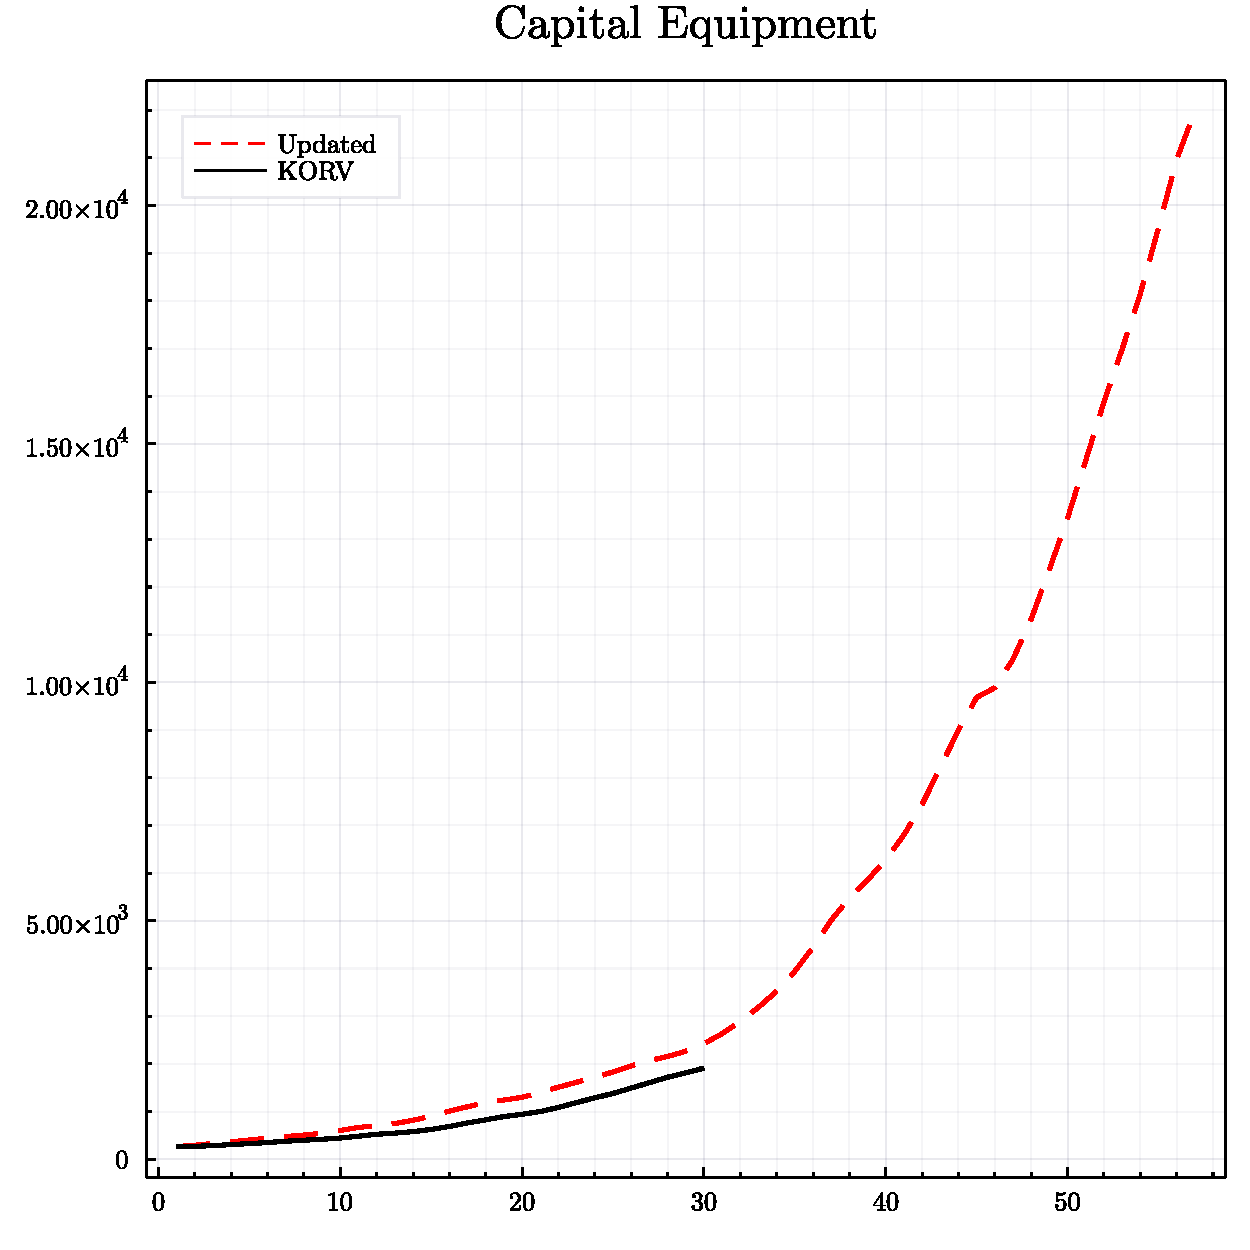
\includegraphics[width=0.3\textwidth]{../images/capital_equipment_doc.pdf}
% \hfill
% 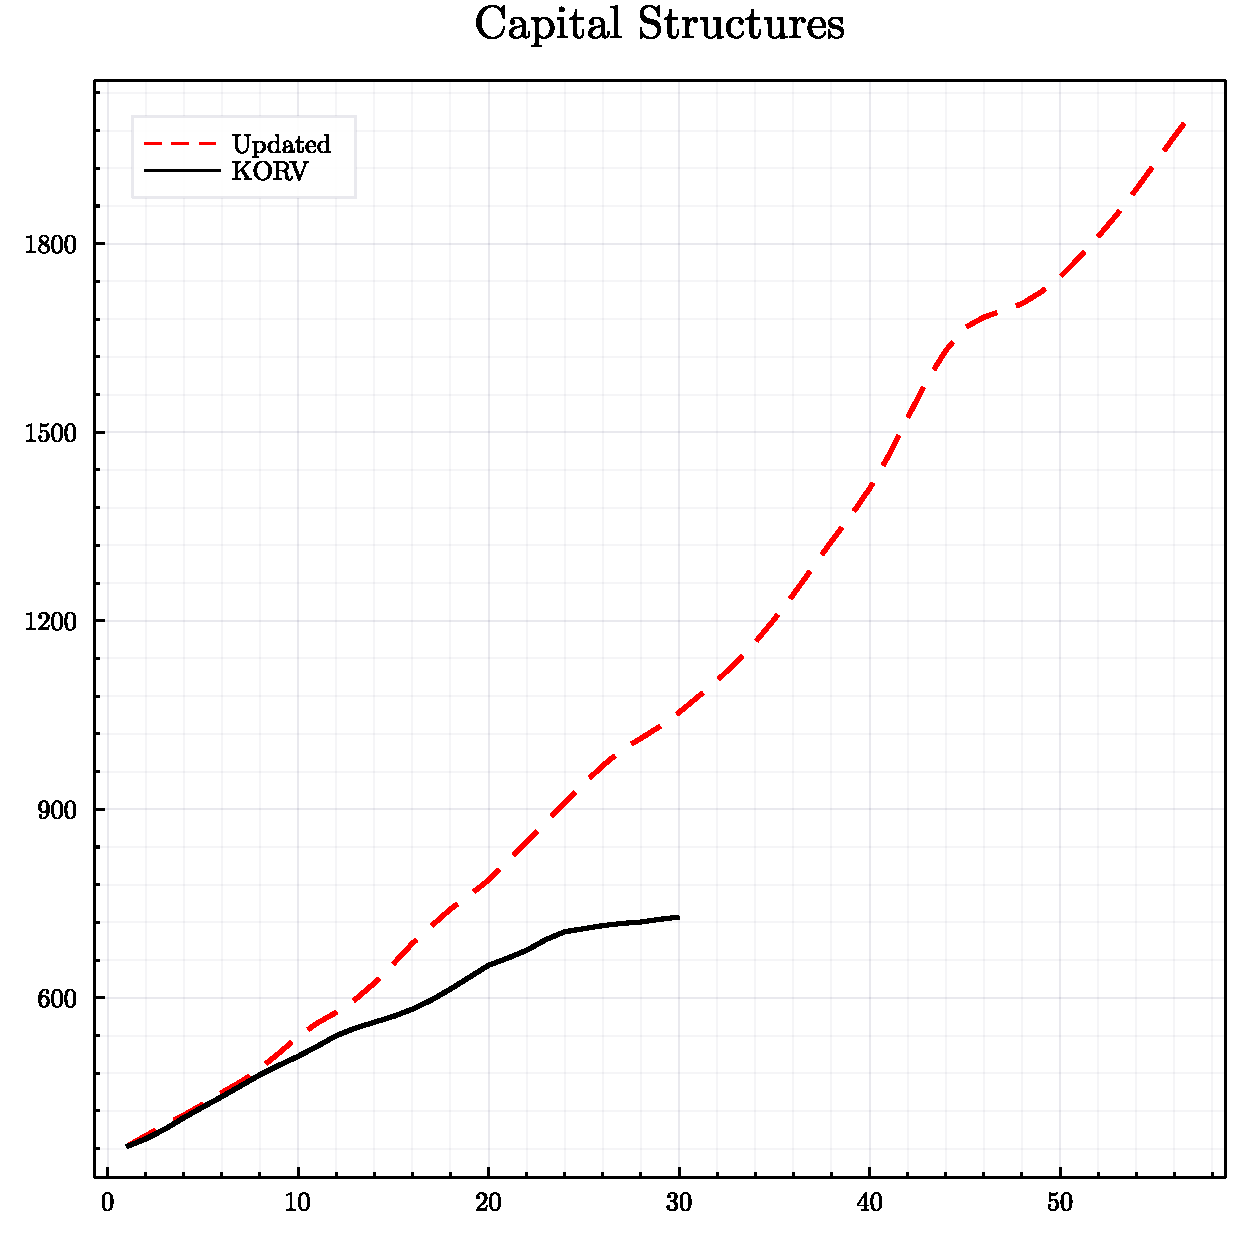
\includegraphics[width=0.3\textwidth]{../images/capital_structures_doc.pdf}
% \hfill
% 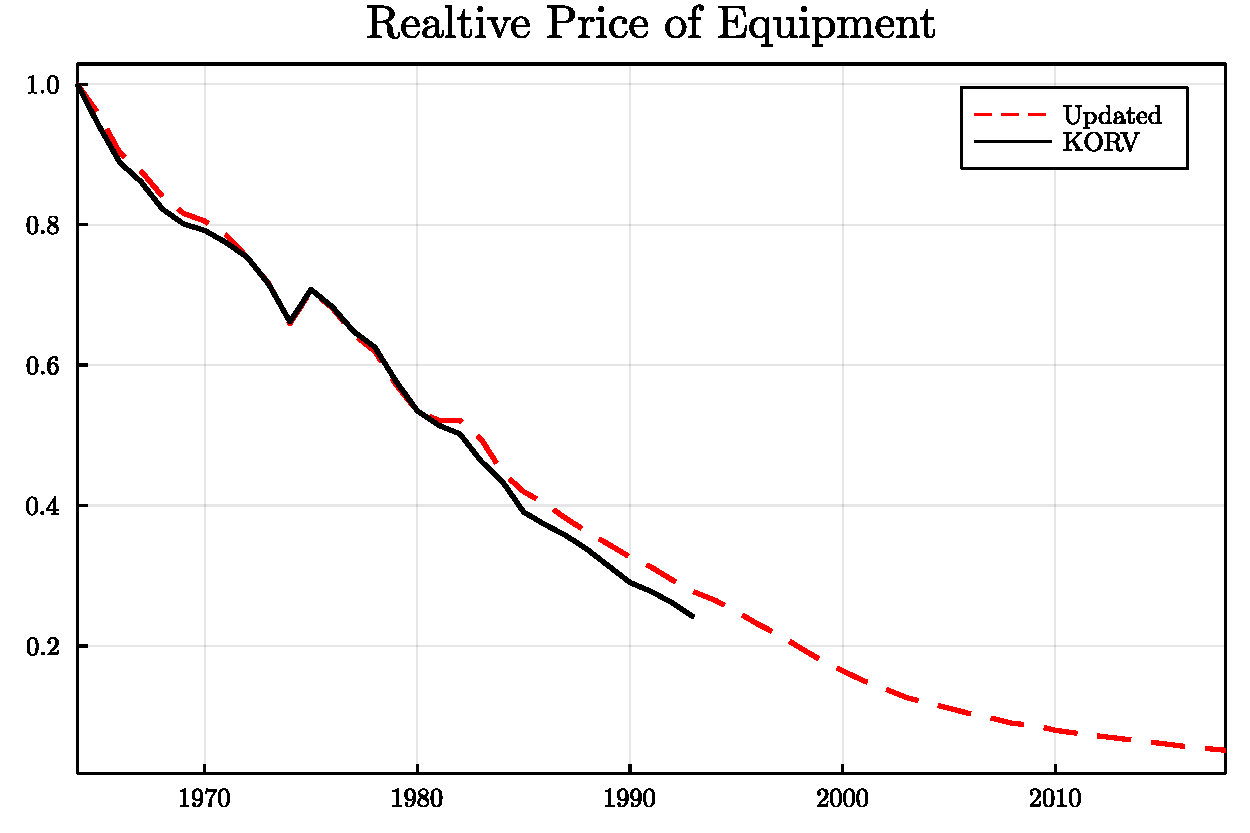
\includegraphics[width=0.3\textwidth]{../images/capital_price_doc.pdf}
% \caption{\label{fig:capital_series} Capital Series}
% \end{figure}

% by \citep{acemoglu2020unpacking}. A description of the codes is in \textcolor{red}{INSER TABLE AND REFERENCEIT}.

% \begin{figure}
% \centering
% 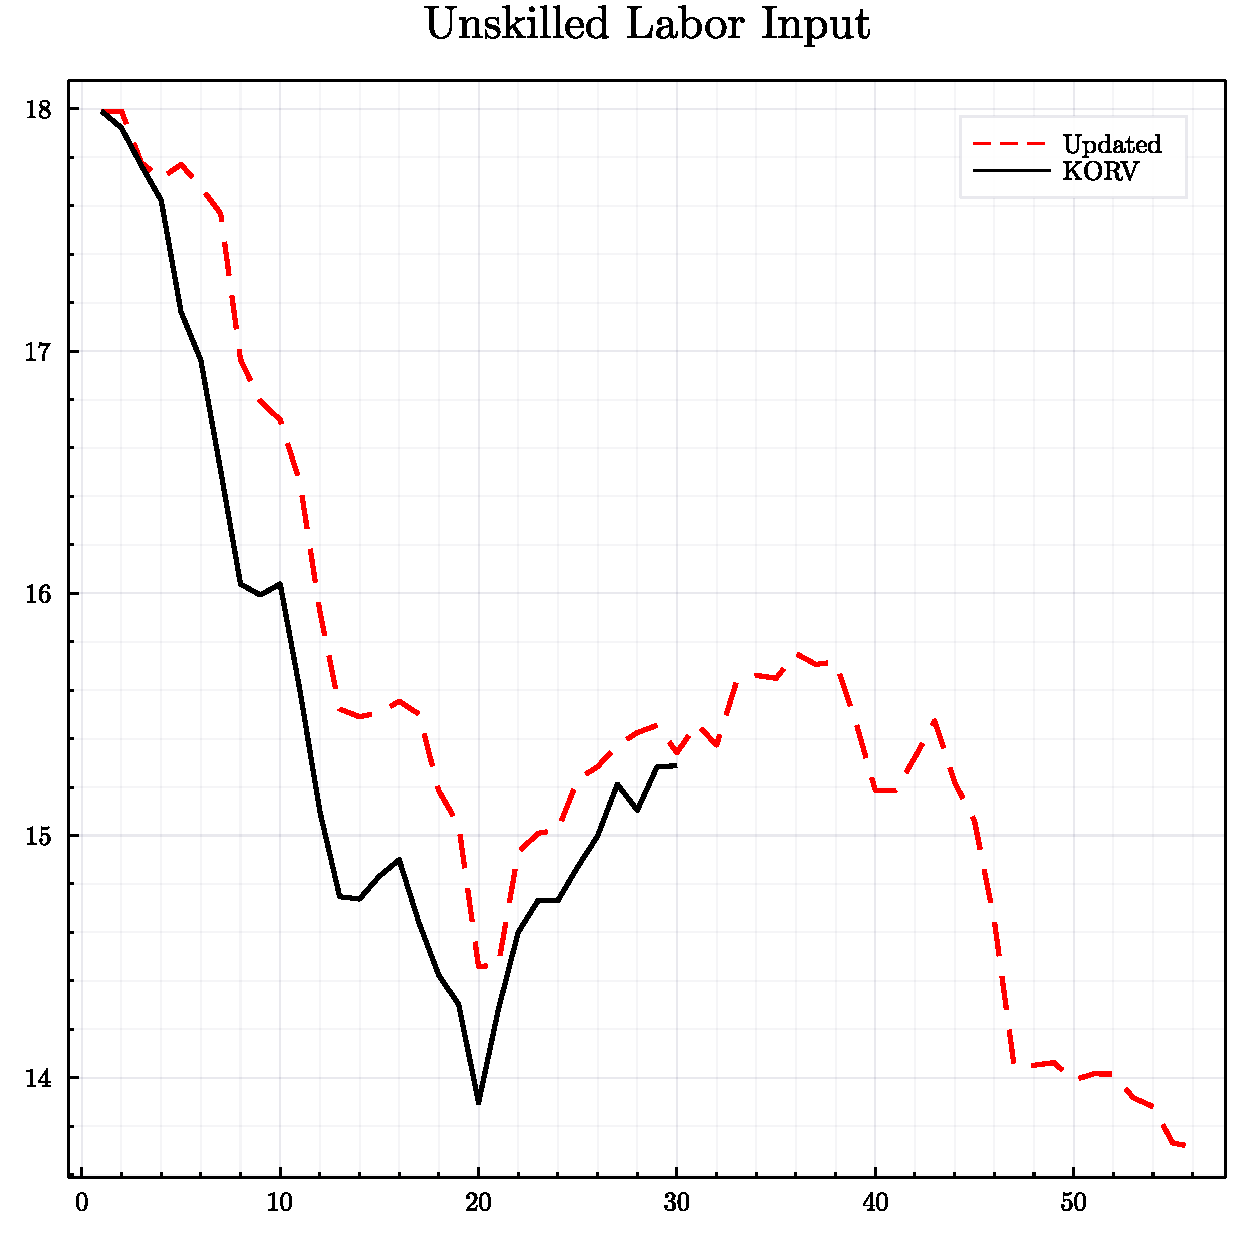
\includegraphics[width=0.45\textwidth]{../images/labor_input_unskilled_doc.pdf}
% \hspace*{0.05\textwidth}
% 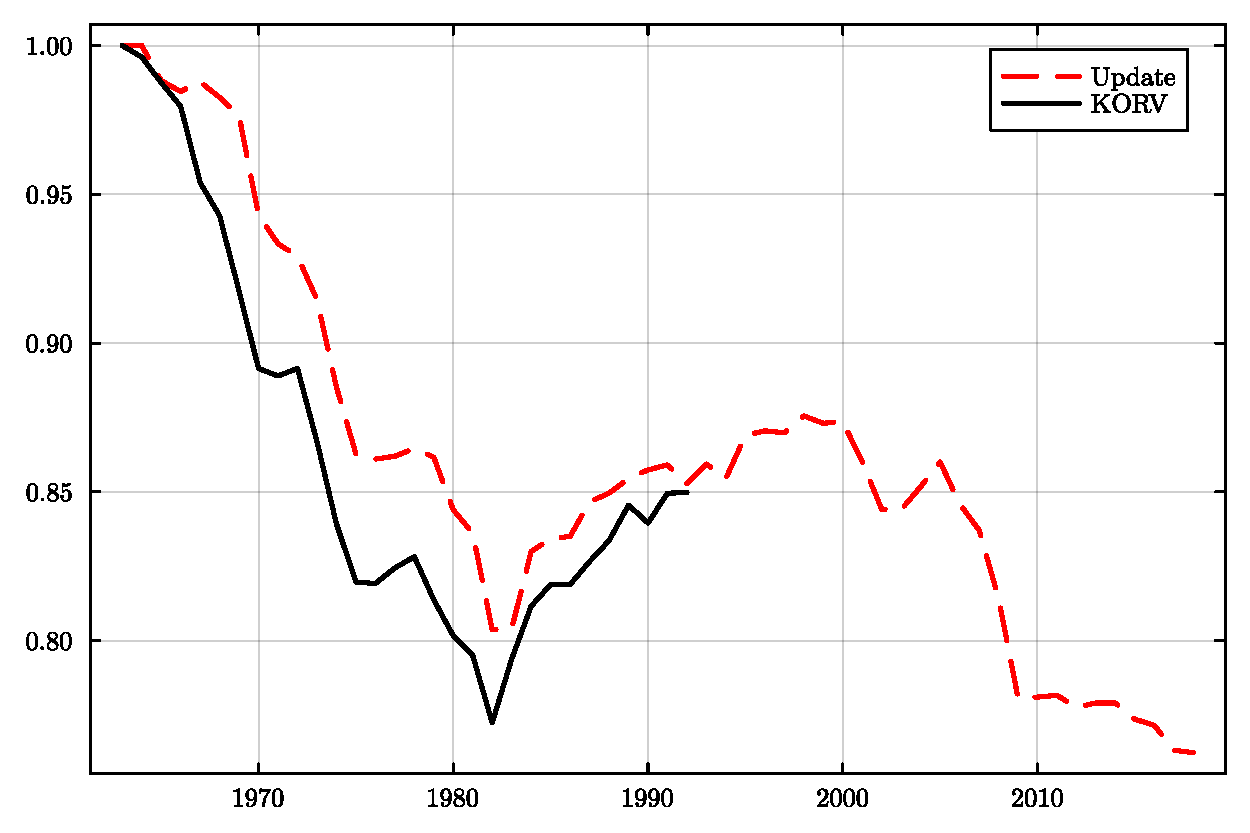
\includegraphics[width=0.45\textwidth]{../images/labor_input_skilled_doc.pdf}
% \vfill
% 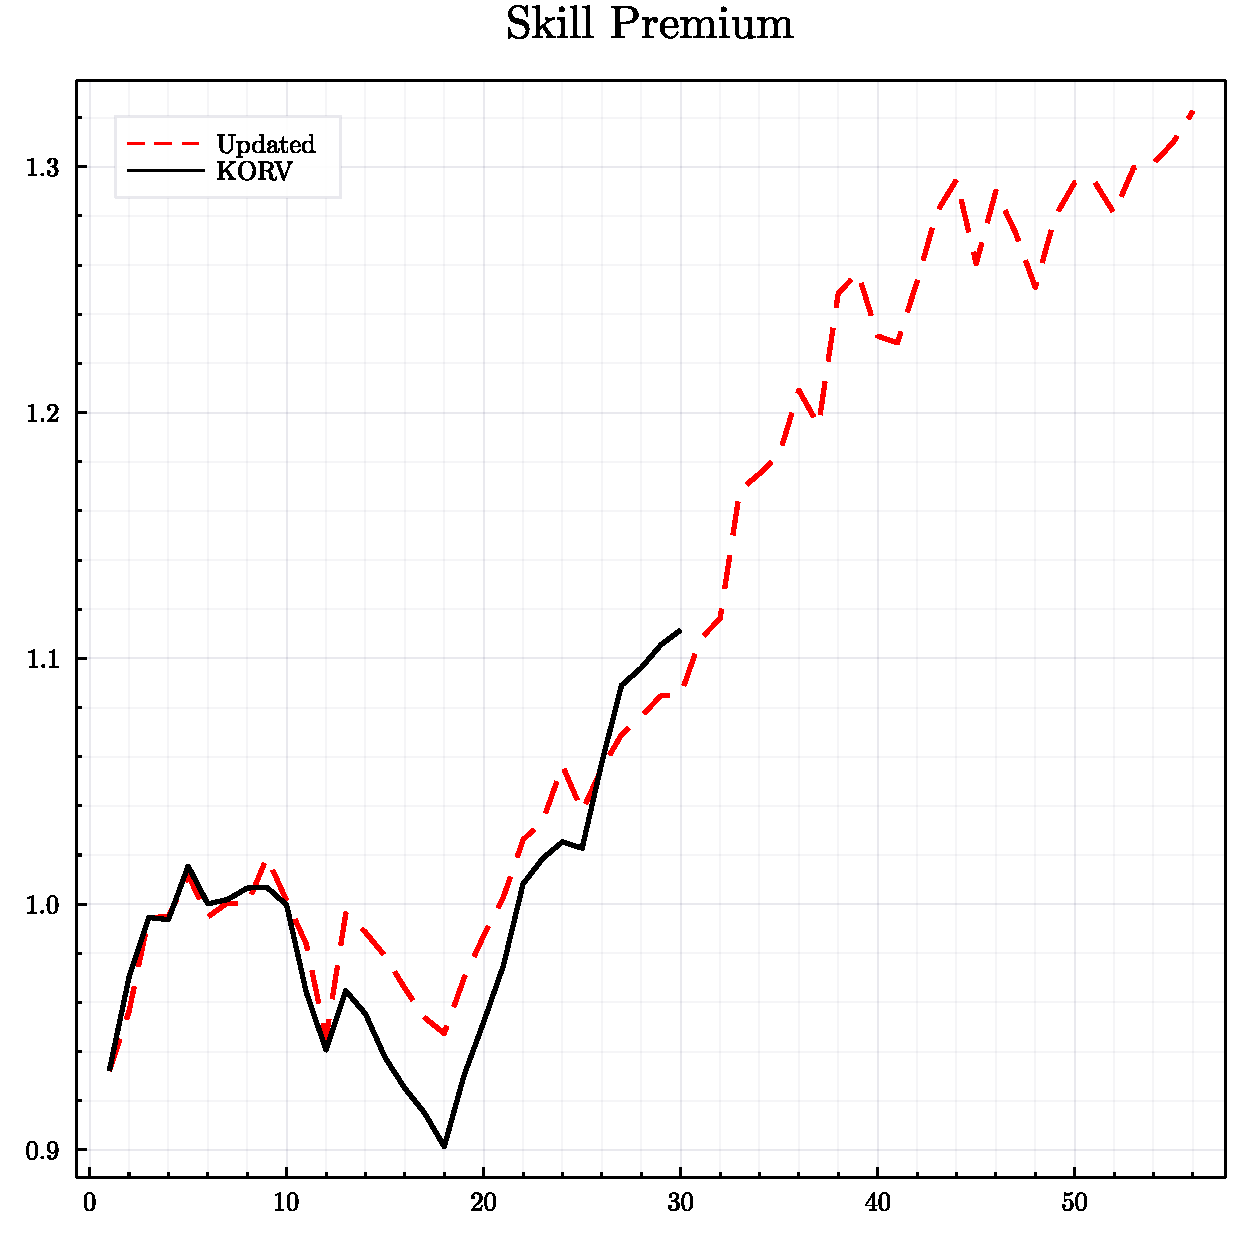
\includegraphics[width=0.45\textwidth]{../images/sp_doc.pdf}
% \hspace*{0.05\textwidth}
% 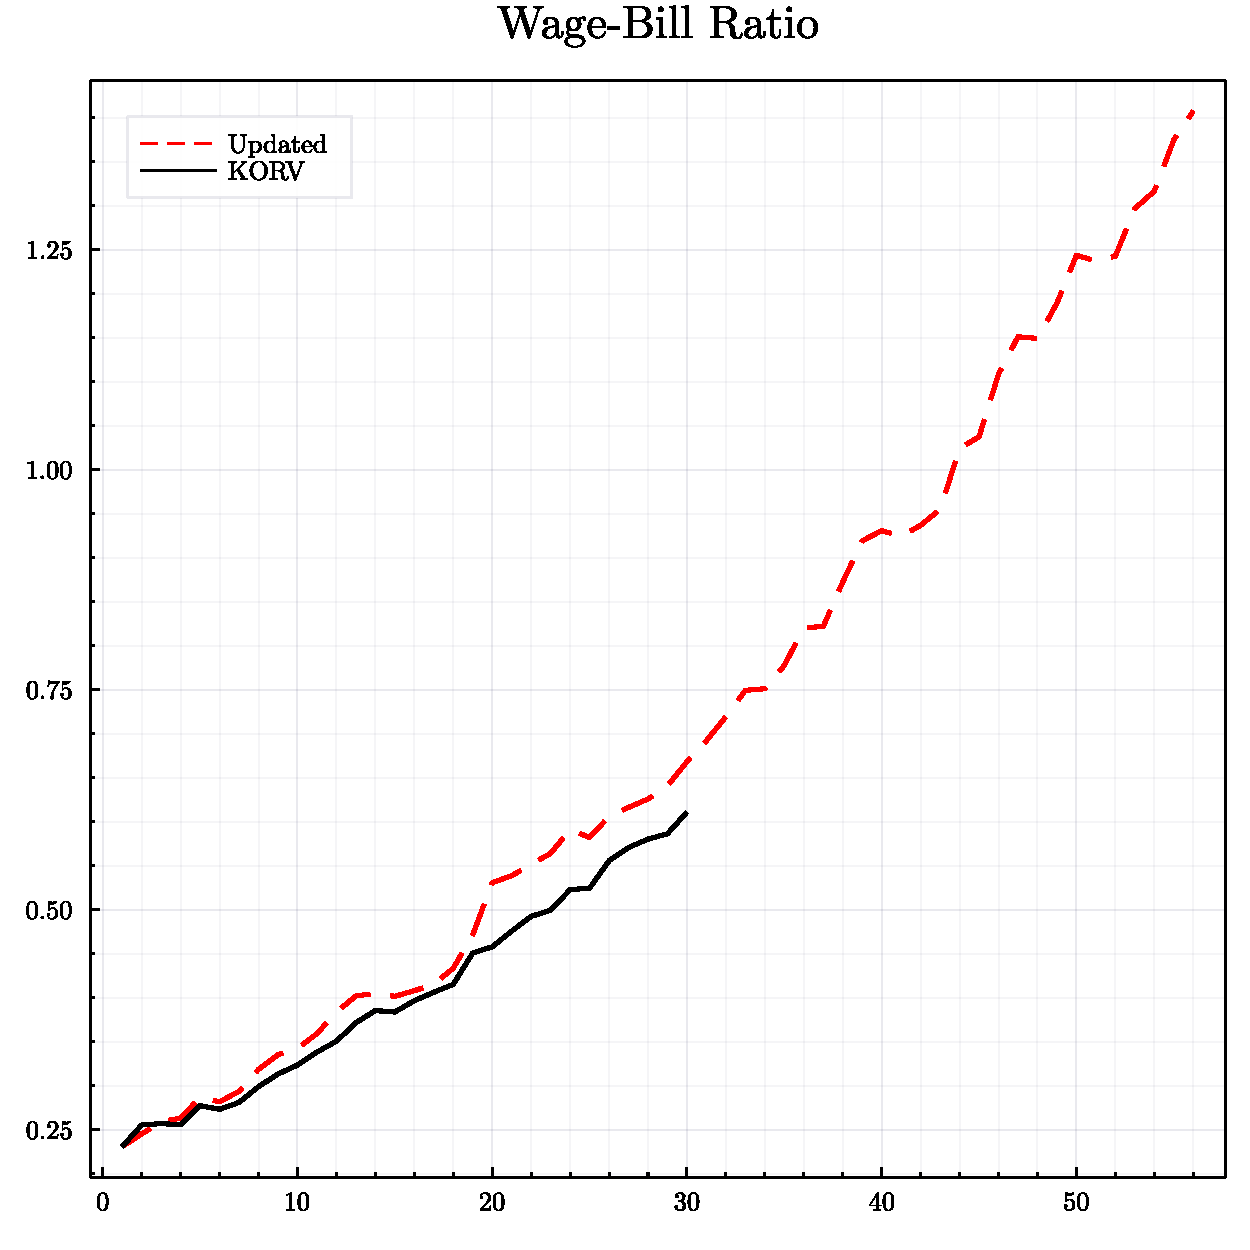
\includegraphics[width=0.45\textwidth]{../images/wbr_doc.pdf}
% \caption{\label{fig:labor_series} Labor Series}
% \end{figure}


% I used the crosswalk in Table \textcolor{red}{INSER TABLE AND REFERENCEIT} to group Census code groups for each industry and subdivided the original CPS data. I then repeated the process described in Appendix~\ref{subsec:labor-inputs-wage-rates} to obtain labor input and wage series for each industry.


% \subsection{Labor Income Shares}\label{sec:labor_share_income}
% To construct labor share series at the economy level I follow \citet{krusell2000capital}, \citet{castex2022decline} and \citet{ohanian2021revisiting} in following the \citet*{cooley1995frontiers}. I first generate a series containing capital income $(CI)$ consisting of the sum of 
% \begin{enumerate}[(i)]
% \item net interest and miscellaneous payments, domestic industries,
% \item corporate profits,
% \item consumption of fixed capital.
% \end{enumerate}
% Capital share is defined as the ratio between $CI$ and gross domestic income (net of proprietors' income) $Y - PI$. Labor share is then calculated as 
% \begin{equation*}
% LI = 1 - \frac{CI}{Y - PI}
% \end{equation*}

% To construct labor share series at the industry level, I used the BEA-BLS Integrated Industry-level Production Accounts (KLEMS). KLEMS dataset contains information on the compensation of employees (with and without a college degree) and the value added by industry, I then follow \citep{karabarbounis2014global} and define the labor share as the ratio between the total compensation of employees and the total value added by industry.

% \begin{figure}[H]
% \centering
% 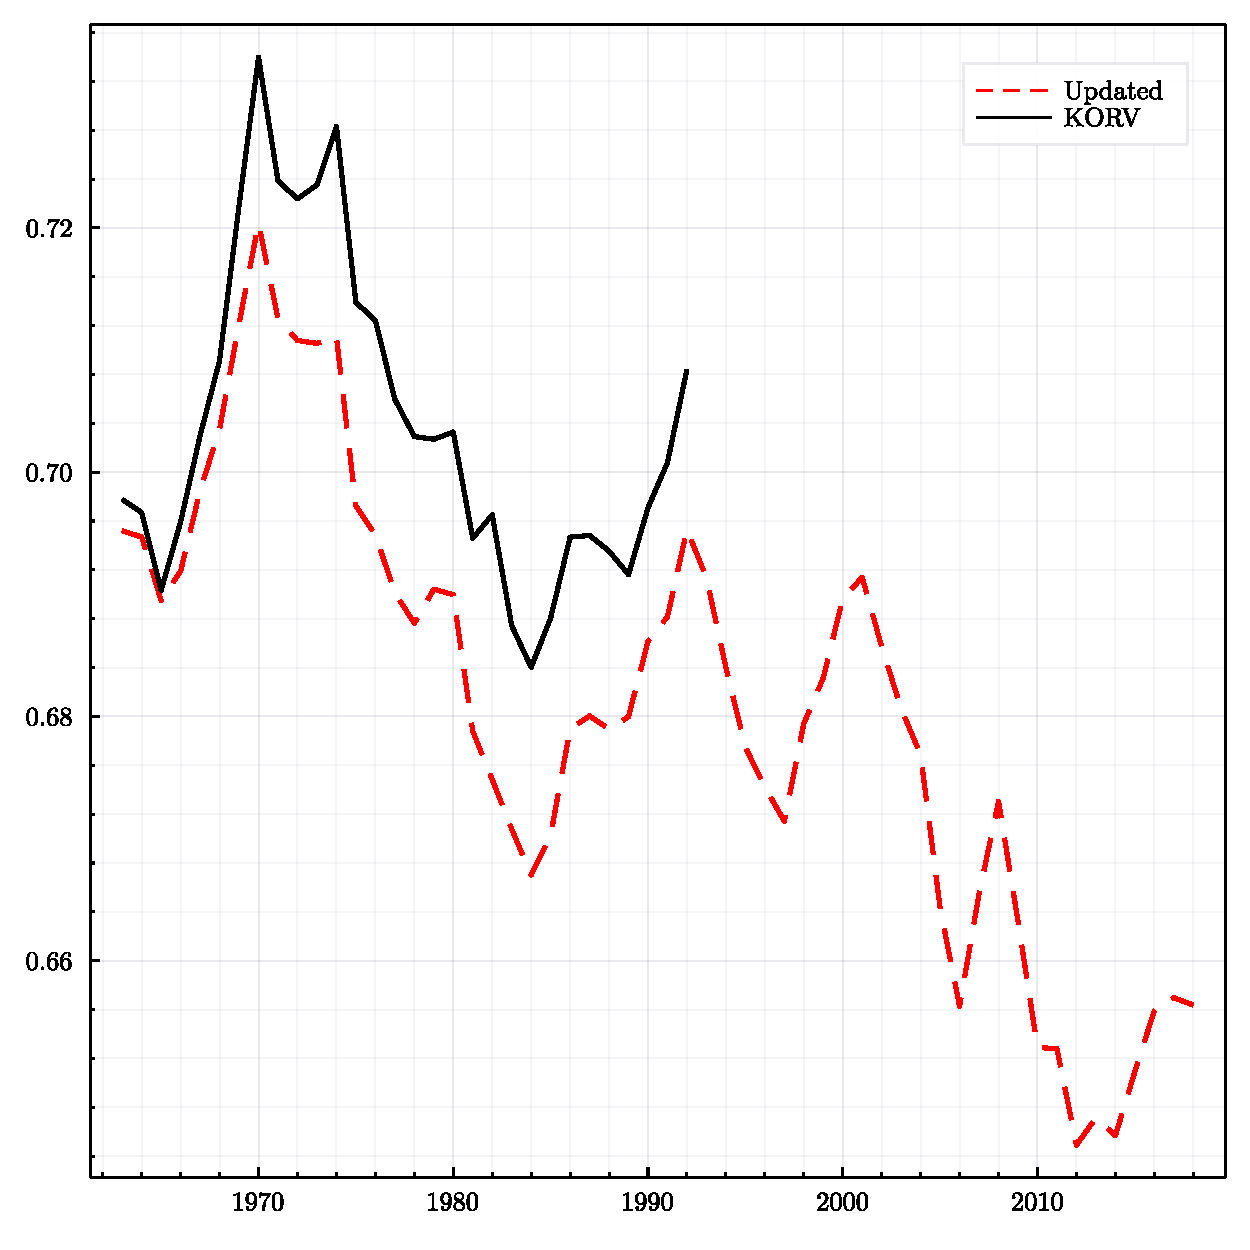
\includegraphics[width=0.5\textwidth]{../images/fig:labor_share_updated.pdf}
% \caption*{\label{fig:labor_share_updated} Labor Share of Income}
% \end{figure}

% \begin{frame}{Industry Level Trends}
% \begin{center}
% \fitimage[]{../images/correlations_wage_LI_slides.pdf}
% \end{center}
% \end{frame}
 

\begin{frame}
 \frametitle{Industry Level Trends}
 \begin{wideitemize}
 \only<1-4>{
 \item To check the relationship between the trends of labor input ratio and the skill premium, I computed the slope of each series in the period:
 }
 \only<2>{
 \begin{figure}[H]
 \centering
 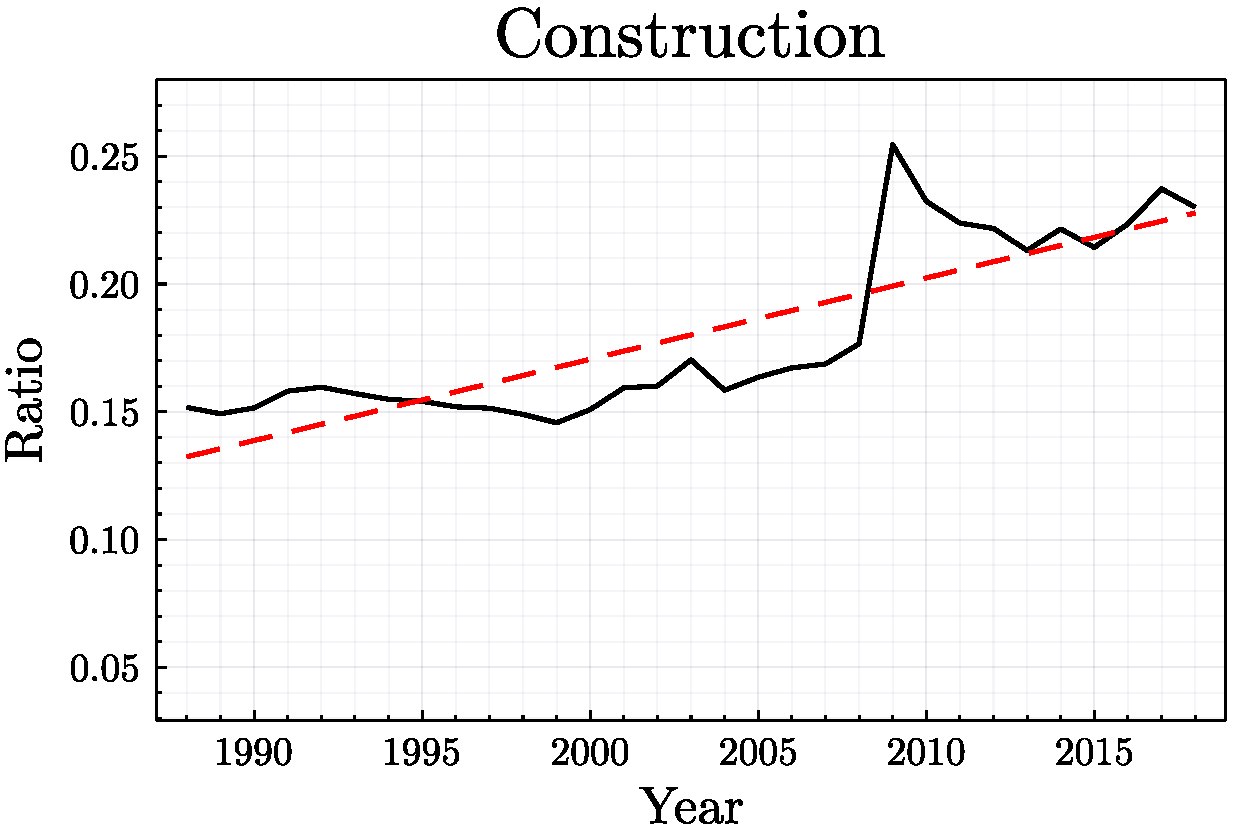
\includegraphics[width=0.4\textwidth]{../images/industries/labor_input_ratio/inc23.pdf}
 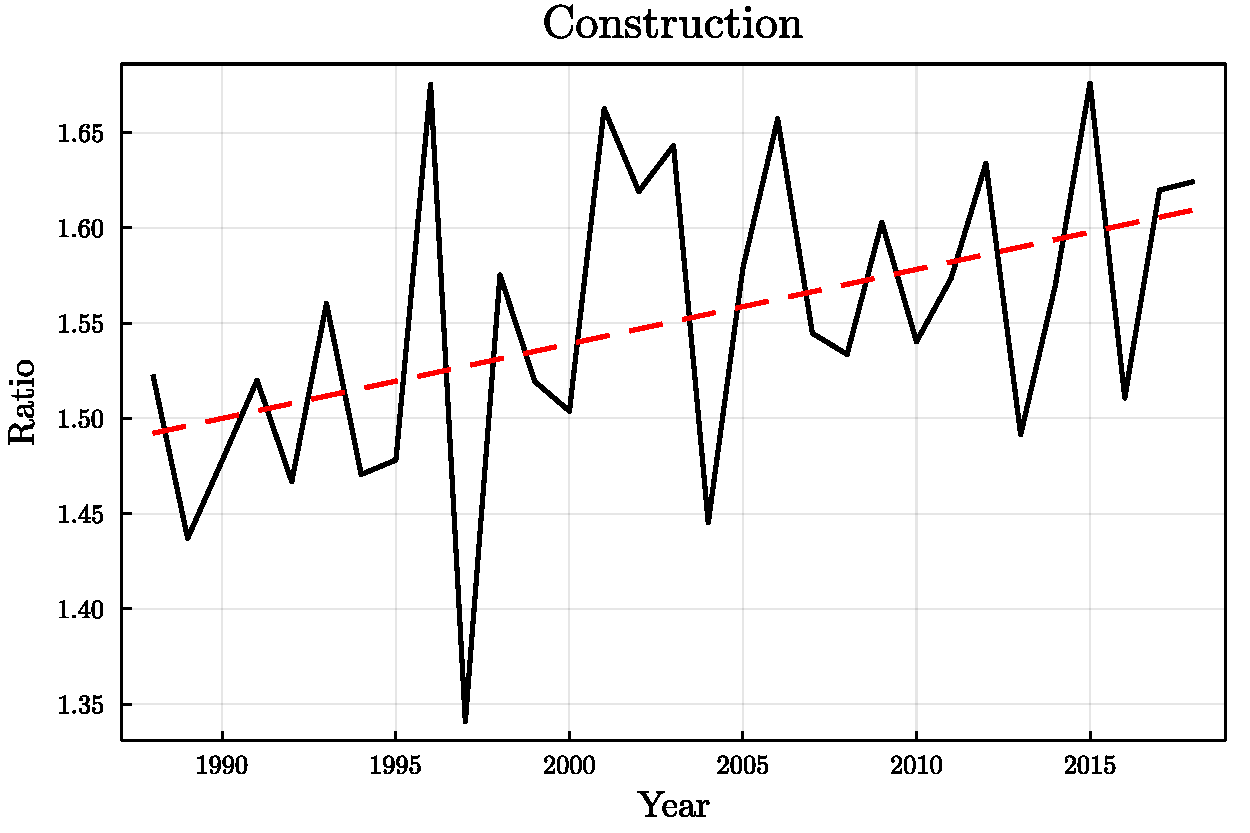
\includegraphics[width=0.4\textwidth]{../images/industries/skill_premium/inc23.pdf}
 \caption{\label{fig:trends_23} Trends: Construction}
 \end{figure}
 }
 \only<3-4>{
 \begin{figure}[H]
 \centering
 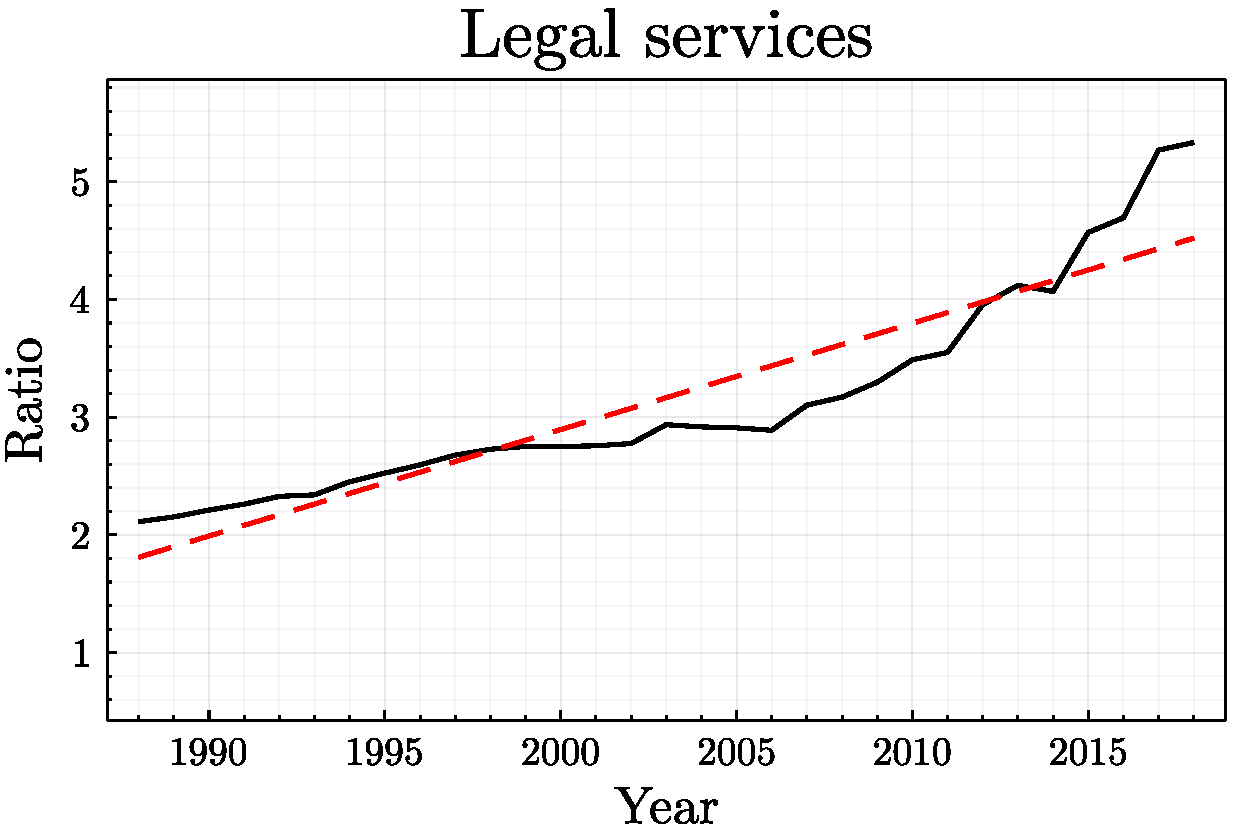
\includegraphics[width=0.4\textwidth]{../images/industries/labor_input_ratio/inc5411.pdf}
 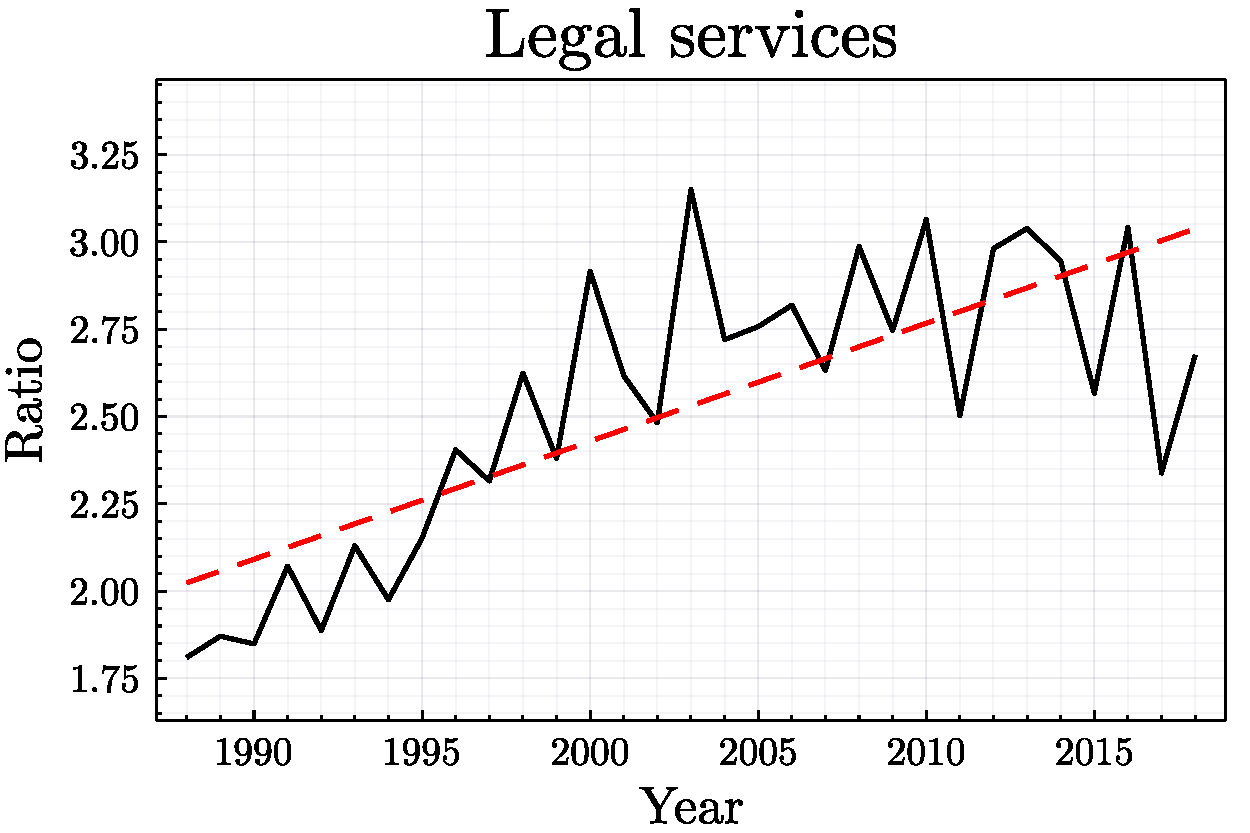
\includegraphics[width=0.4\textwidth]{../images/industries/skill_premium/inc5411.pdf}
 \caption{\label{fig:trends_5411} Trends: Legal Services}
 \end{figure}
 }
 \only<4>{
 \item For $49$ industries ($87.5\%$)the skill premium increased in the period and the input ratio showed the same pattern for $52$ ($92.8\%$) industries.
 }
 \end{wideitemize}
\end{frame}

\begin{frame}{Industry Level Trends \hyperlink{sp-model-decomposition}{\beamergotobutton{Back}}}\label{frame-industry-trends}

 \fitimage[Realtionship between the trends of Labor Input and Skill Premium. $84\%$ of the industries are increasing in both. ]{../images/trend_correlation_slides.pdf}

\end{frame}

\section{Model}
\begin{frame}{KORV}
 \begin{wideitemize}
 \item Two types of capital
 \begin{itemize}
 \item $k_s$, structures.
 \begin{itemize}
 \item Buildings.
 \end{itemize}
 \item $k_e$, equipment, with a relative price equal to $1/q$
 \begin{itemize}
 \item Machines, computers, intellectual property.
 \end{itemize}
 \end{itemize}
 \item Two types of labor
 \begin{itemize}
 \item $u$ low-skilled labor.
 \begin{itemize}
 \item $u= \psi^u h_u$ where $h_u$ is hours (observed) and $\psi^u$ is the quality of low-skilled labor (unobserved). 
 \end{itemize}
 \item $s$ high-skilled labor.
 \begin{itemize}
 \item $s = \psi^S h_s$ where $h_s$ is hours (observed) and $\psi^s$ is the quality of high-skilled labor (unobserved). 
 \end{itemize}
 \end{itemize}
\end{wideitemize}
\end{frame}

\begin{frame}{KORV}
 \begin{wideitemize}
 \item There are three final goods:
 \begin{itemize}
 \item Consumption $c$
 \item Structure investment $i_s$
 \item Equipment investment $i_e$.
 \end{itemize}
 \item Aggregate production:
 \begin{equation}\label{eq:production}
 c_t + i_{e_t} + i_{s_t} = Y_t = A_t G(k_{s_t}, k_{e_t}, u_t, s_t)
 \end{equation}
 \end{wideitemize}
\end{frame}

\begin{frame}{Production function}
 \begin{wideitemize}
 \item The production function is:
 \begin{equation}\label{eq:production_fun}
 G(k_{s_t}, k_{e_t}, u_t, s_t) = k_{s_t}^\alpha\left( \mu u_t^\sigma + (1-\mu)\left(\lambda k_{s_t}^\rho (1-\lambda)s_t^\rho\right)^\frac{\sigma}{\rho}\right)^\frac{1-\alpha}{\sigma}
 \end{equation}
 \item $\sigma_{H} = 1/(1-\rho)$ is the elasticity between equipment and high-skilled.
 \item $\sigma_{L} = 1/(1-\sigma)$ is the elasticity between low-skilled and equipment + high-skilled.
 \item Firms solve the following profit maximization problem 
 \begin{equation}\label{eq:profit_max}
 \max_{k_{s_t}, k_{e_t}, u_t, s_t} G(k_{s_t}, k_{e_t}, u_t, s_t) - r_{s_t}k_{s_t} - r_{e_t}k_{e_t} - w_{u_t} h_{u_t} - w_{s_t} h_{s_t}
 \end{equation}
 \end{wideitemize}
\end{frame}

\begin{frame}{Production Function}
 \begin{wideitemize}
 \item My objective is to use this model to test whether the evolution of the change in the wage premium for skilled labor in different industries can be explained using the capital-skill complementarity hypothesis.
 
 % % \only<2->{
 \item I can observe, $\textcolor{black}{w_{u}}, \textcolor{black}{w_{s_t}}, k_{s_t}, \textcolor{black}{k_{e_t}}, \textcolor{black}{h_{u_t}}, \textcolor{black}{h_{s_t}}$
 % % }
 % % \only<3->{
 % \item $H = \psi_t^H h$ and $L = \psi_t^L \ell$ where $\textcolor{black}{\psi_t^H}, \textcolor{black}{\psi_t^L}$, are assumed to be a random process $\psi_t^i = \psi_0^i + \varepsilon$. \only<4->{ With $\epsilon\sim\mathcal{N}(0, \textcolor{black}{\eta}) $}
 % % }
 % % \only<4->{
 % \item $\textcolor{black}{\sigma}, \textcolor{black}{\rho}$ and $\textcolor{black}{\eta}$, I take from original paper (for now).
 % % }
 % % \only<5->{
 % \item Finally I estimate $\textcolor{black}{\lambda}, \textcolor{black}{\psi_0^H}$ and $\textcolor{black}{\psi_0^L}$, using \textbf{SPML} method.
 % % }
 
 \end{wideitemize}
\end{frame}

\subsection{Skill-Premium}
\begin{frame}{Skill Premium in the Model}
 % \only<1->{
 % Define skill premium ($\omega$) as the ratio of the wages of skilled to unskilled.
 
 \begin{wideitemize}
 \item Assuming competitive markets, workers are paid their marginal products per unit, of work:
 % }
 \begin{equation*}
 \omega_t = \frac{w_{s_t}}{w_{u_t}} = \frac{G_{h_s}(k_{s_t}, k_{e_t}, u_t, s_t) }{G_{h_u}(k_{s_t}, k_{e_t}, u_t, s_t) }
 \end{equation*}
 % \only<3->{
 \item We can obtain the following (log-linearized) expression for $\omega_t$:
 \begin{equation}\label{eq:skill_premium_log_linear}
 \ln \omega_{t} \simeq \lambda \frac{\sigma-\rho}{\rho}\left(\frac{k_{e_t}}{s_{t}}\right)^{\rho}+(1-\sigma) \ln \left(\frac{h_{u_t}}{h_{s_t}}\right)+\sigma \ln \left(\frac{\psi^s_t}{\psi^u_t}\right)
 \end{equation}
 \item Which in turn can be written in terms of growth rates ($g_x$):
 \begin{equation}\label{eq:skill_premium_growth_rates}
 \begin{aligned}
 g_{\omega t} \simeq &(1-\sigma)\left(g_{h_{u_t}}-g_{h_{s_t}}\right)+\sigma\left(g_{\psi^s_t}-g_{\psi^u_t}\right) \\
 &+(\sigma-\rho) \lambda\left(\frac{k_{e_t}}{s_{t}}\right)^{\rho}\left(g_{k_{e_t}}-g_{h_{s_t}}-g_{\psi^s_t}\right) 
 \end{aligned}
 \end{equation}
 \end{wideitemize}
\end{frame}

\begin{frame}{Skill Premnium Decomposition}\label{sp-model-decomposition}
 
 We have decomposed the skill premium into three parts:
 \begin{wideitemize}
 \vspace{0.5cm}
 \only<1>{
 \item $(1-\sigma)(g_{h_{u_t}}-g_{h_{s_t}})$ depends on the difference of the growth rates of skilled and unskilled and labor.
 \vspace{0.5cm}
 \begin{wideitemize}
 \item If both types of labor are substitutes i.e $\sigma_u < 0 \implies (1-\sigma) < 0$
 \item If skilled labor grows at a faster rate than unskilled labor, then the skill premium decreases. \hyperlink{frame-industry-trends}{\beamerbutton{Data}}
 \end{wideitemize} 
 }\only<2>{
 \item $\sigma\left(g_{\psi^s_t}-g_{\psi^u_t}\right)$ depends on the growth rate of the productivity of skilled and unskilled and labor. 
 \vspace{0.5cm}
 \begin{wideitemize}
 \item I follow KORV in making the following stochastic assumptions about labor productivity:
 \begin{equation}\label{eq:stochastic_labor_productivity}
 \psi^i_t = \psi^i_0 + \epsilon \qquad \epsilon \sim N(0, \eta_\omega^2) \qquad i\in\{s,u\}
 \end{equation}
 \item On average $\sigma (g_{\psi^s_t}-g_{\psi^u_t} )$ is constant over time and does not affect the growth rate of the skill premium.
 \end{wideitemize} 
 }\only<3>{
 \item $(\sigma-\rho) \lambda\left(\frac{k_{e_t}}{s_{t}}\right)^{\rho}\left(g_{k_{e_t}}-(g_{h_{s_t}}+g_{\psi_{s_t}})\right)$. This component depends on two factors:
 \vspace{0.5cm}
 \begin{enumerate}
 \item The growth rate of equipment relative to the growth rates of skilled labor input.
 \vspace{0.5cm}
 \begin{wideitemize}
 \item Characterize the capital-skill complementarity hypothesis as $\sigma > \rho$.
 \item If equipment capital grows faster than skilled labor, the skill-premium will increase.
 \end{wideitemize}
 \vspace{0.5cm}
 \item The ratio of capital equipment to skilled labor 
 \vspace{0.5cm}
 \begin{wideitemize}
 \item The effect will get larger (smaller) over time if $\rho > 0\:$ ($\rho < 0$). 
 \end{wideitemize}
 \end{enumerate} 
 }
\end{wideitemize}
\end{frame}

\section{Estimation}
\begin{frame}
 \frametitle{Estimation}

 \begin{wideitemize}
 \item I follow the same methodology as KORV to estimate the model parameters.
 \only<1>{
 \item To simplify notation :
 \begin{align*}
 \psi_t &= \{\psi^u_t, \psi^s_t\} \\
 X_t &= \{ k_{s_t} , k_{e_t}, h_{s_t}, h_{u_t}\} \\
 \Phi &= \{\alpha, \sigma, \rho, \mu, \lambda, \psi^u_0, \psi^s_0, \eta_\omega \}
 \end{align*}
 \item Any $\{\mu, \lambda, \psi^u_0,\mu, \lambda, \psi^u_0, \psi^s_0\}$ act as scaling parameters thus, one can be fixed.
 \item There are $7$ parameters to be estimated.
 }\only<2>{
 \item The parameters are estimated using the following structural equations:
 \begin{align*}
 A_{t+1} G_{k_s}(X_{t+1}, \psi_{t+1} \mid \Phi ) &= q_t A_{t+1} G_{k_s}(X_{t+1}, \psi_{t+1} \mid \Phi ) + (1-\delta_e)\left(\frac{q_t}{q_{t+1}}\right) + \nu_t\\
 \frac{w_{s_t}h_{s_t} + w_{u_t}h_{u_t} }{Y_t} &= lsh(X_{t}, \psi_{t} \mid \Phi ) \\
 \frac{w_{s_t}h_{s_t}}{w_{u_t}h_{u_t}} &= wbr(X_{t}, \psi_{t} \mid \Phi )
 \end{align*}
 }\only<3>{
 \item The estimation method is a two-stage simulated pseudo-maximum likelihood estimation (SPMLE).
 \item In the first stage labor input is considered to be endogenous and is instrumented using: both capital series, lagged capital series, lagged prices, and indicators of the business cycle.
 \item In the second stage:
 \begin{wideitemize}
 \item Taking the variance $\eta_\omega$ as given, for each date $t$, generate $S$ realizations of the model.
 \item For each date $t$ calculate the mean and variance of the realizations.
 \item Minimize the distance between the first moments of the model and the data, using the second moment as a weighting matrix.
 \end{wideitemize}
 }
 \end{wideitemize}

\end{frame}

\section{Results}
\begin{frame}
 \frametitle{Results}
 \begin{wideitemize}
 \item First, I will show the results of the replication of the model using updated data.
 \item Second, I will show the results of applying the model to each industry.
 \end{wideitemize}
\end{frame}

\subsection{KORV Replication}
\begin{frame}
 \frametitle{KORV Replication}
 \only<1>{
 \begin{table}[h]
 \begin{center}
 \begin{tabular}{rrrrr}
  \hline\hline
   & \textbf{KORV Estimation} & \textbf{Replication} & \textbf{Updated Data} & \textbf{Updated Data} \\
   & \texttt{$1963$ - $1992$} & \texttt{$1963$ - $1992$} & \texttt{$1963$ - $2018$} & \texttt{$1988$ - $2018$} \\\hline
  $\alpha$ & 0.117 & 0.113 & 0.118 & 0.08 \\
  $\sigma$ & 0.401 & 0.464 & 0.503 & 0.313 \\
  $\rho$ & -0.495 & -0.56 & -0.343 & -0.154 \\
  $\eta_\omega$ & 0.043 & 0.043 & 0.083 & 0.043 \\\hline\hline
\end{tabular}

 \caption{\label{tab:estimation_korv} Parameter estimates KORV model.}
 \end{center}
 \end{table}
 }\only<2>{
 % \begin{table}[h]
 % \begin{center}
 % \begin{tabular}{rrrrr}
  \hline\hline
   & \textbf{KORV Estimation} & \textbf{Replication} & \textbf{Updated Data} & \textbf{Updated Data} \\
   & \texttt{$1963$ - $1992$} & \texttt{$1963$ - $1992$} & \texttt{$1963$ - $2018$} & \texttt{$1988$ - $2018$} \\\hline
  $\sigma_s$ & 0.668896 & 0.641107 & 0.744831 & 0.857268 \\
  $\sigma_u$ & 1.66945 & 1.86506 & 2.01136 & 1.8599 \\\hline\hline
\end{tabular}

 % \caption{\label{tab:estimation_elasticities_korv} Implied Elastities of Substitution}
 % \end{center}
 % \end{table}

 \begin{figure}[H]
 \centering
 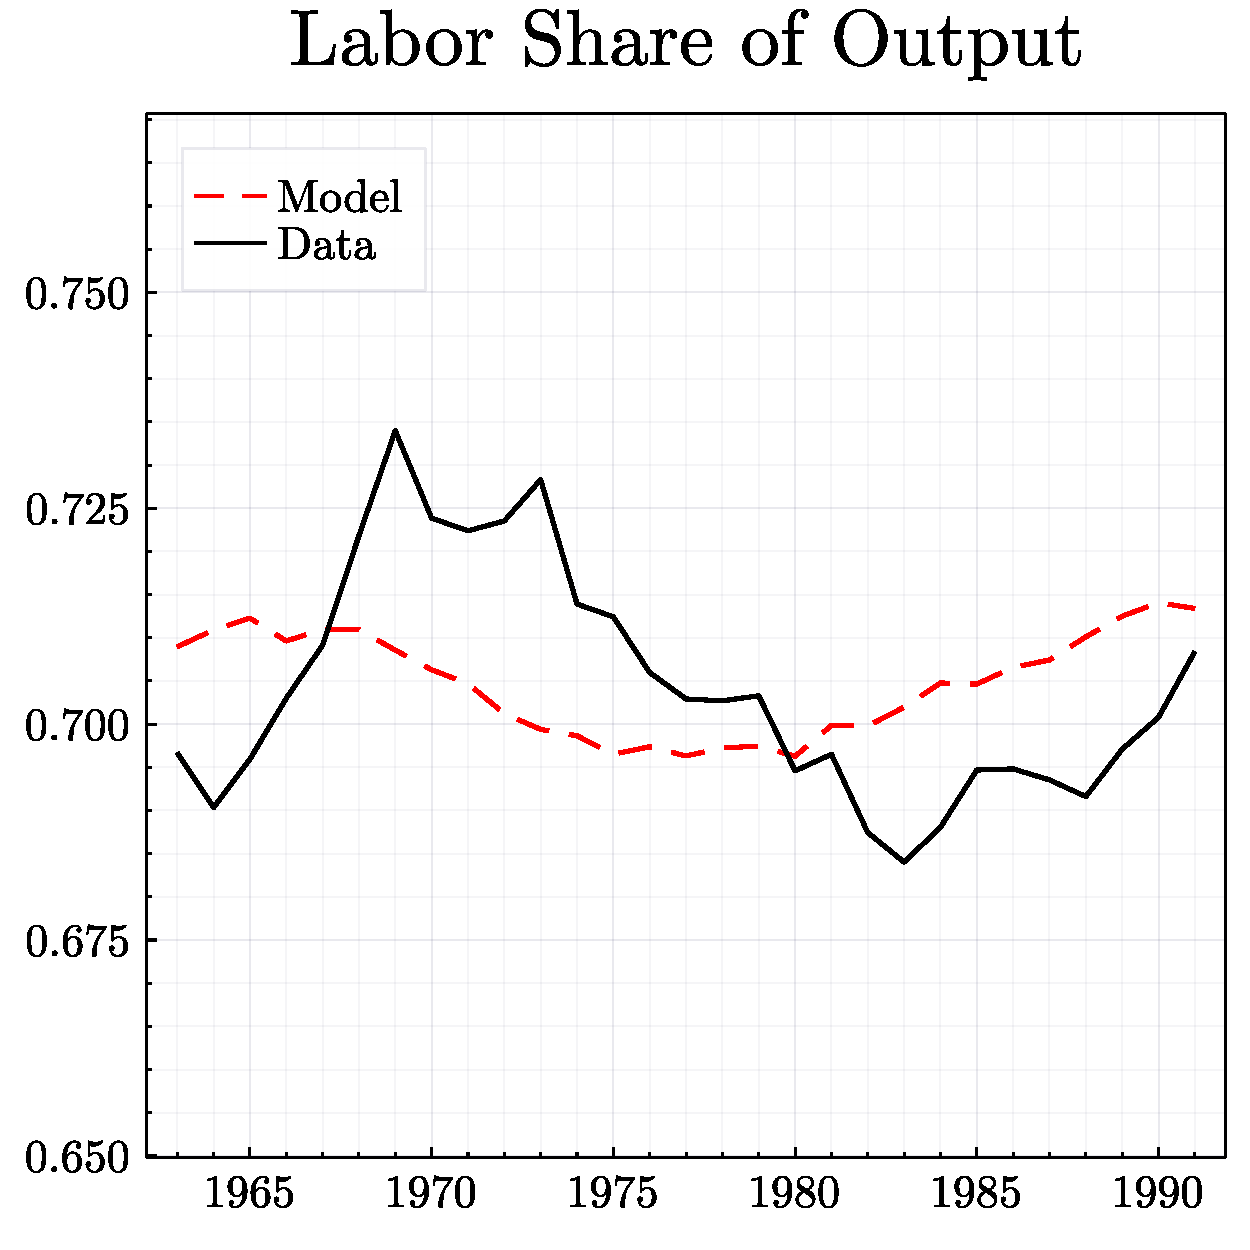
\includegraphics[width=0.3\textwidth]{../images/fig:korv_estimation_ls_slides.pdf}
 \hfill
 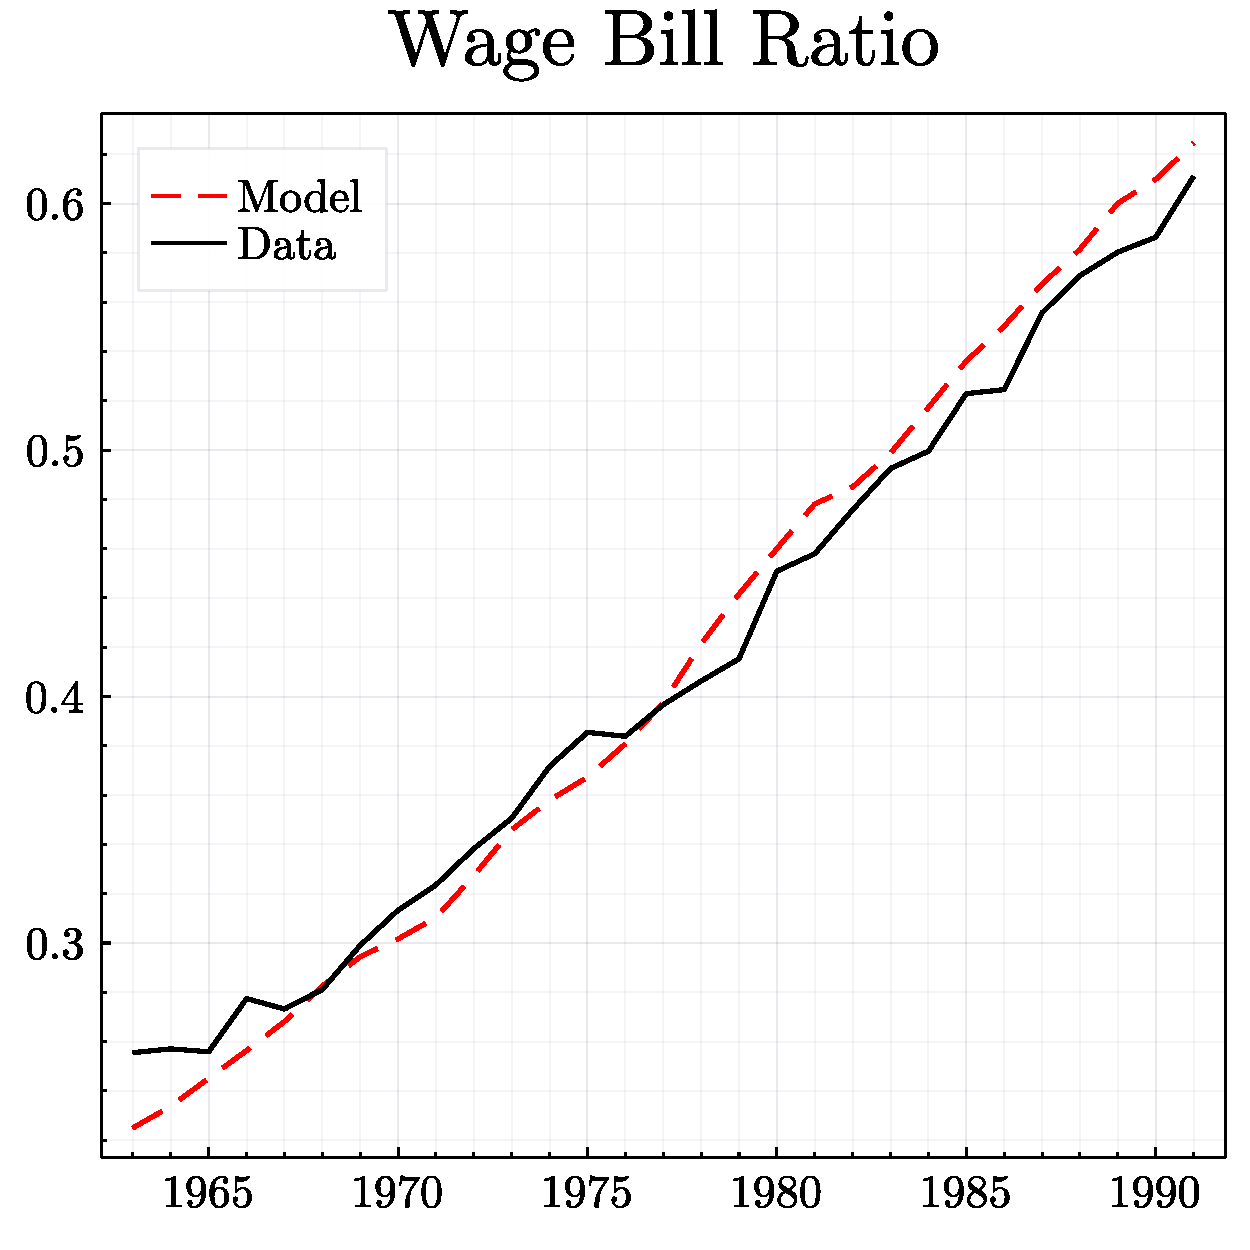
\includegraphics[width=0.3\textwidth]{../images/fig:korv_estimation_wbr_slides.pdf}
 \hfill
 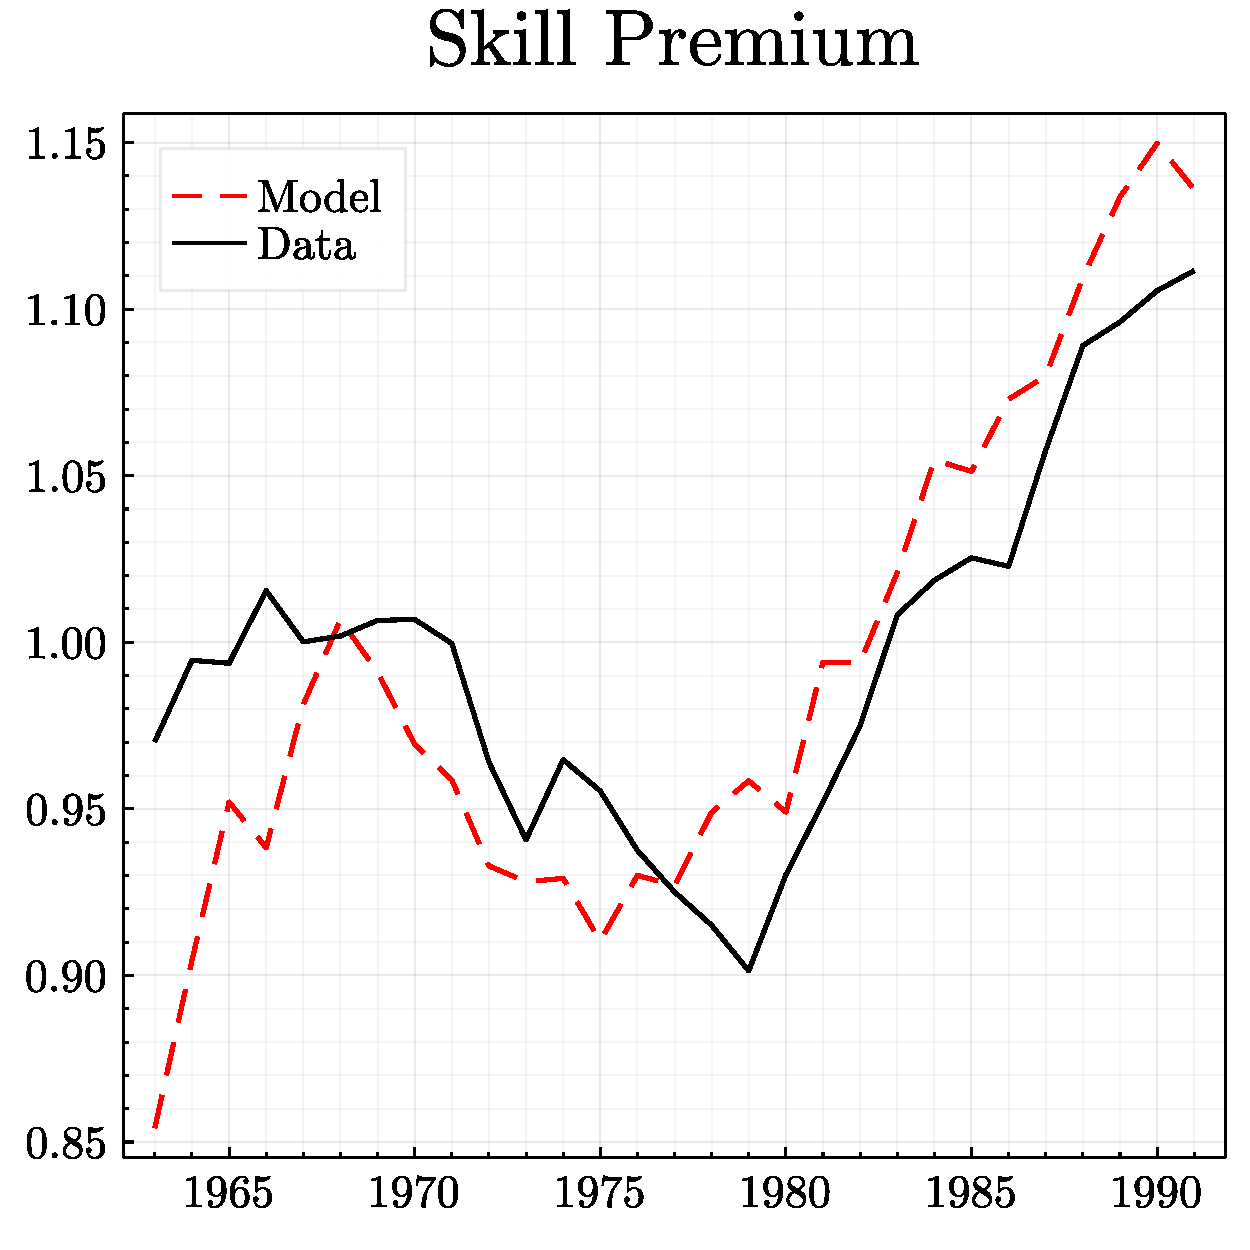
\includegraphics[width=0.3\textwidth]{../images/fig:korv_estimation_sp_slides.pdf}
 \caption{\label{fig:korv_estimation} Fit for the $1963$ - $1992$ period with KORV Data.}
 \end{figure}
 }\only<3>{
 \begin{figure}[H]
 \centering
 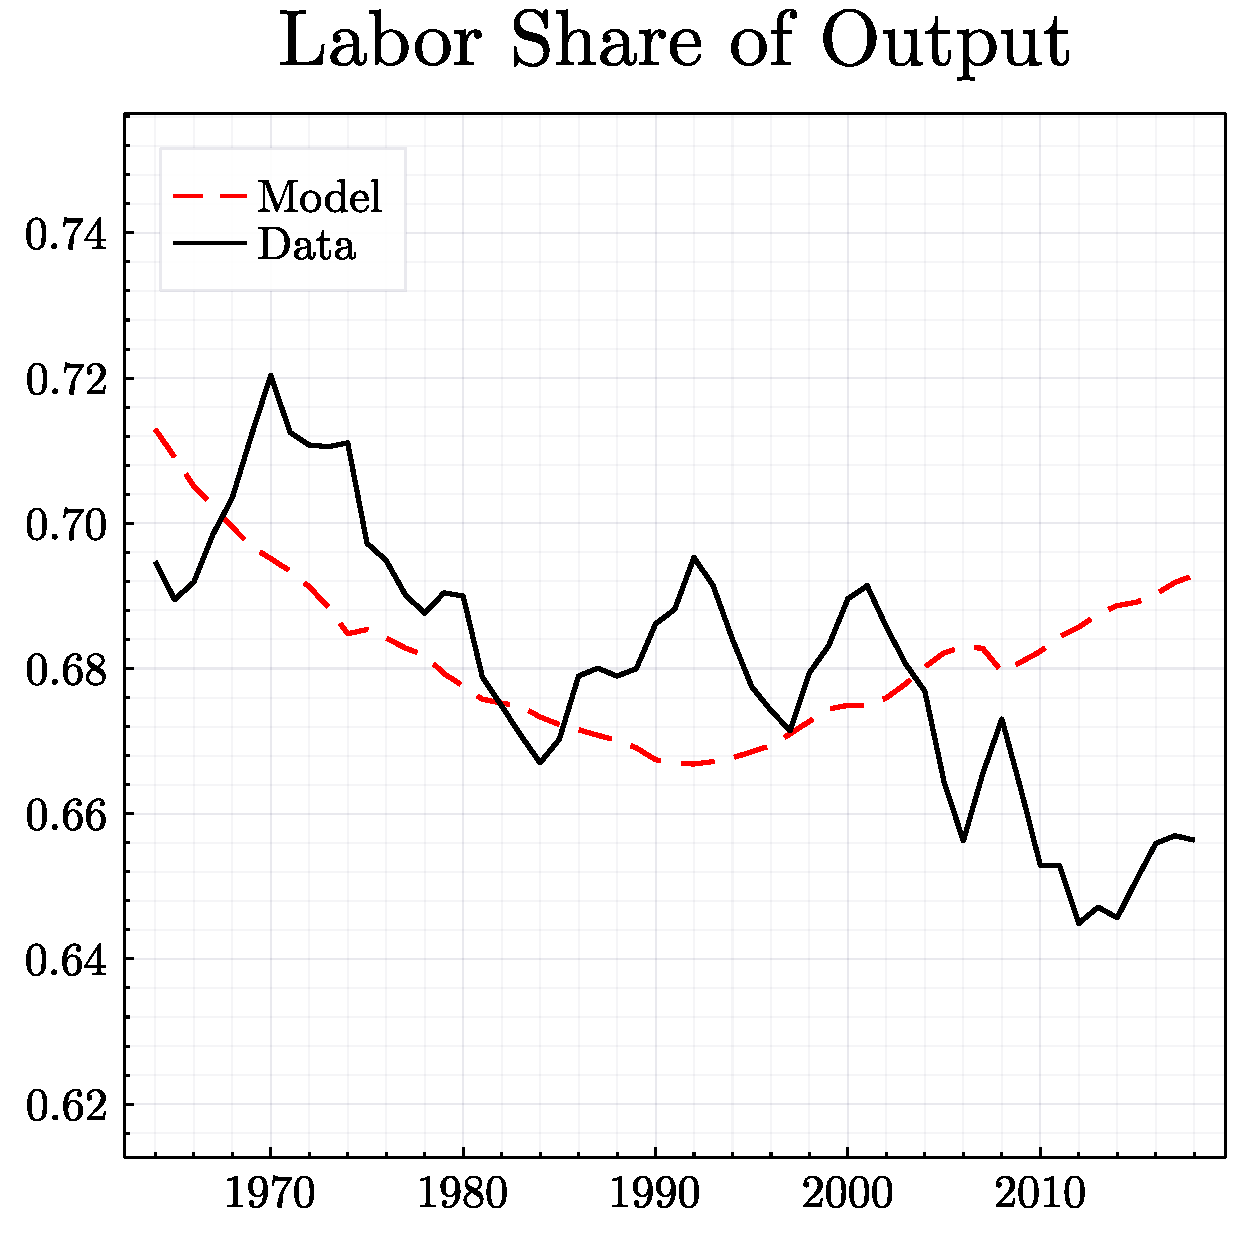
\includegraphics[width=0.3\textwidth]{../images/fig:updated_estimation_ls_slides.pdf}
 \hfill
 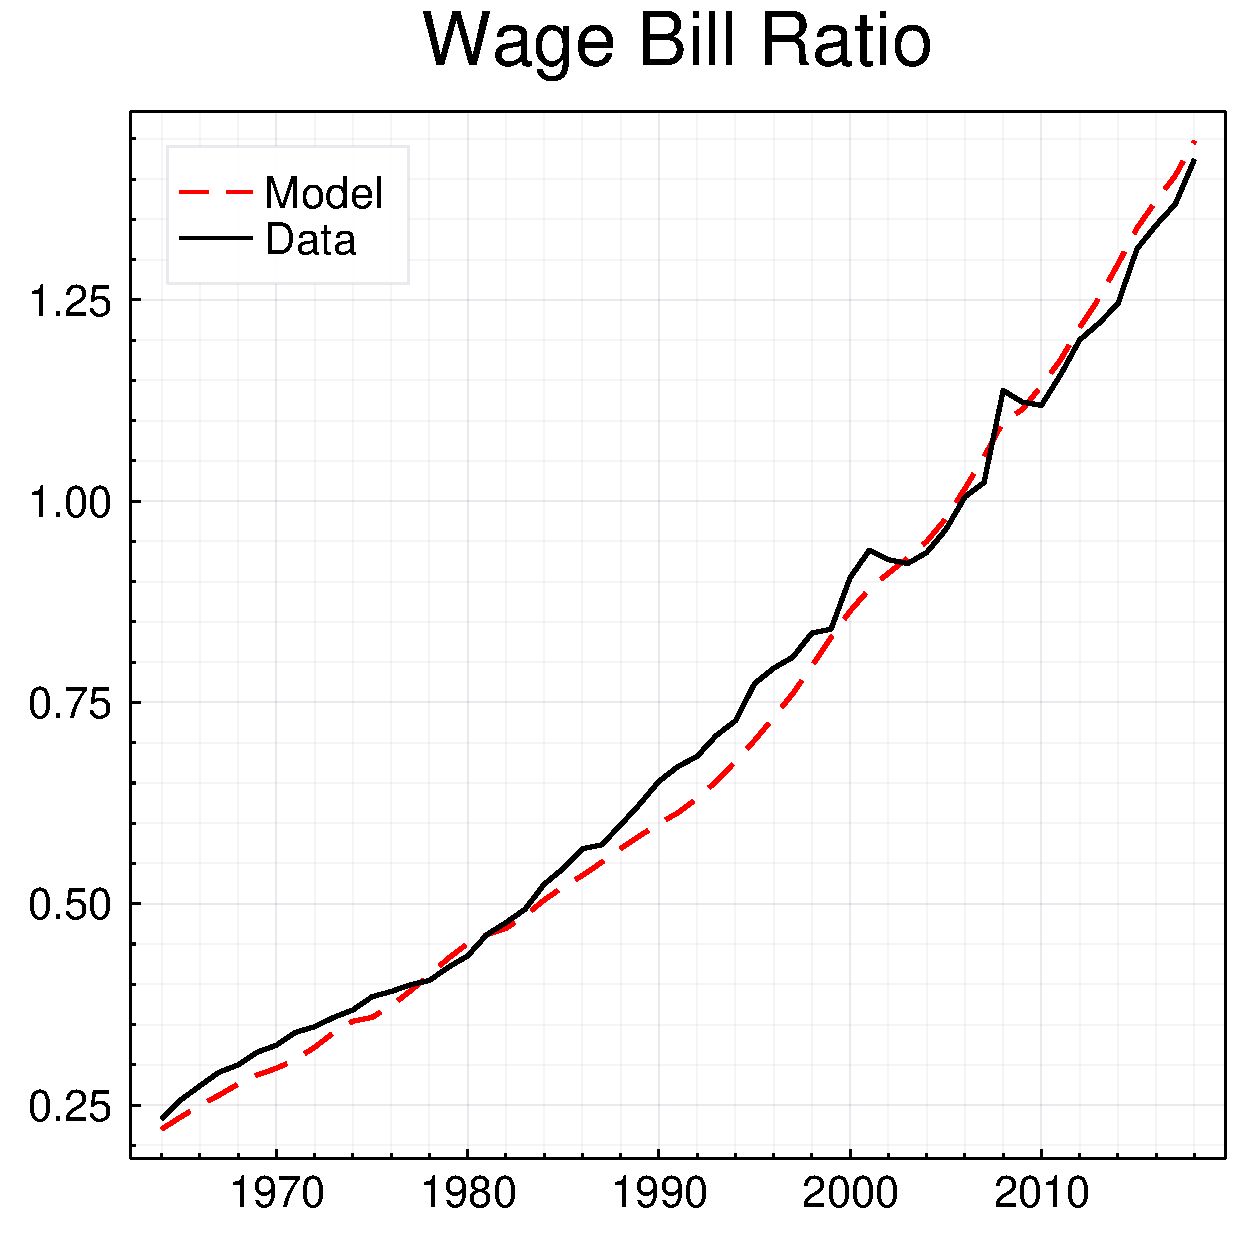
\includegraphics[width=0.3\textwidth]{../images/fig:updated_estimation_wbr_slides.pdf}
 \hfill
 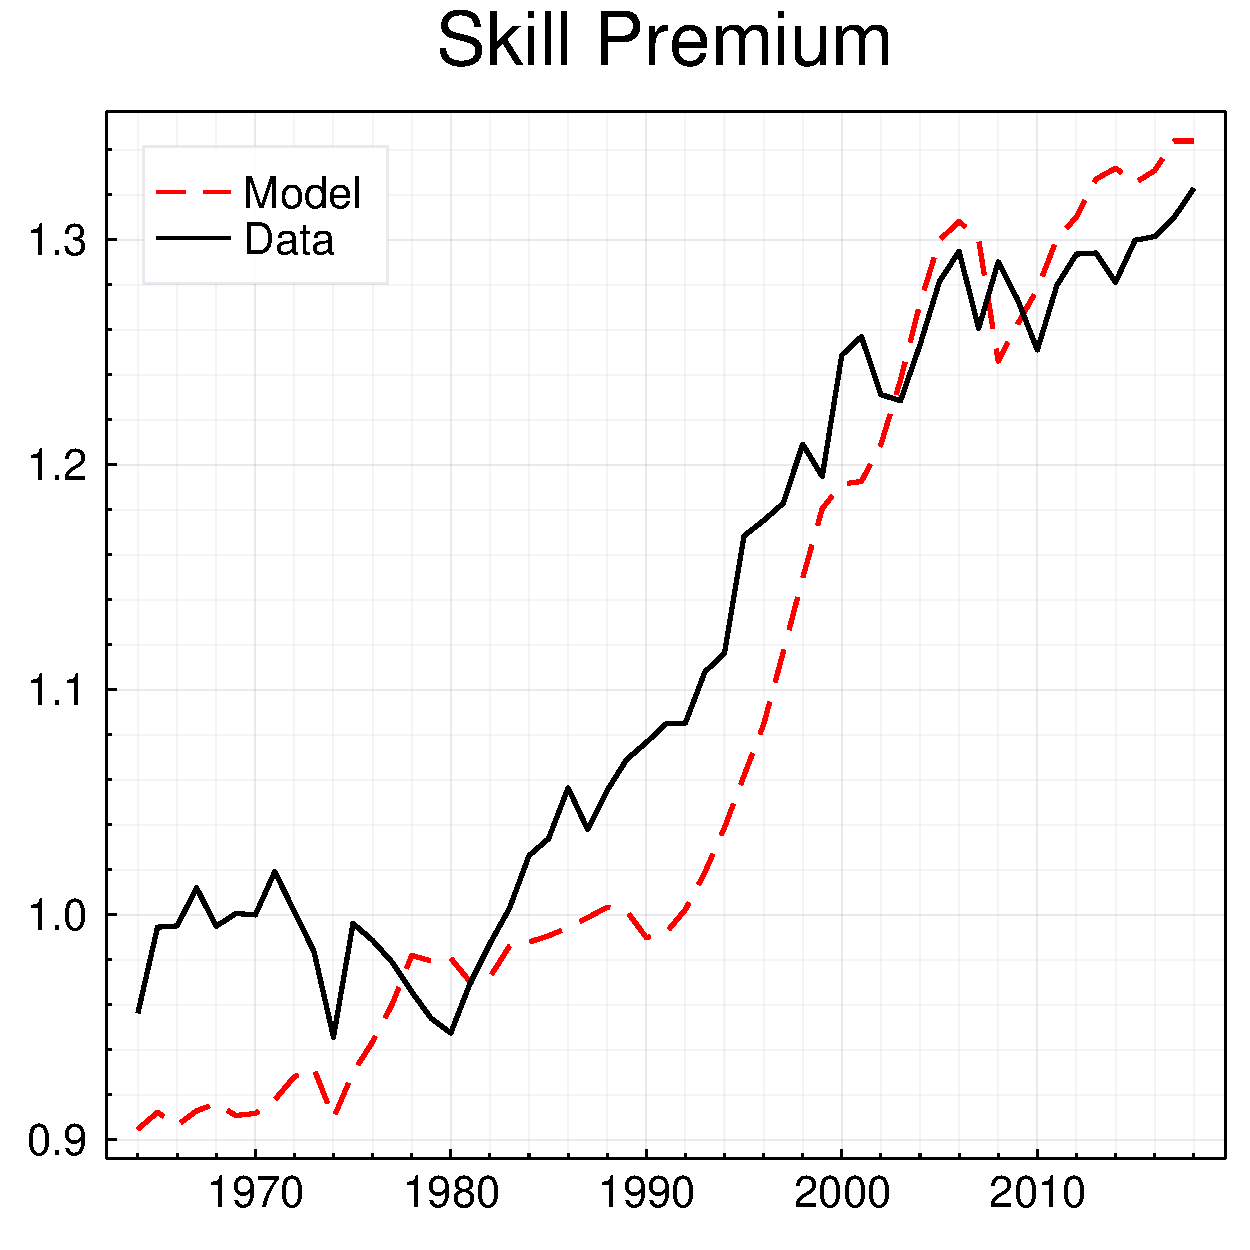
\includegraphics[width=0.3\textwidth]{../images/fig:updated_estimation_sp_slides.pdf}
 \caption{\label{fig:korv_estimation_extended} Fit for the $1963$ - $2018$ period with Updated Data.}
 \end{figure}
 }\only<4>{
 \begin{figure}[H]
 \centering
 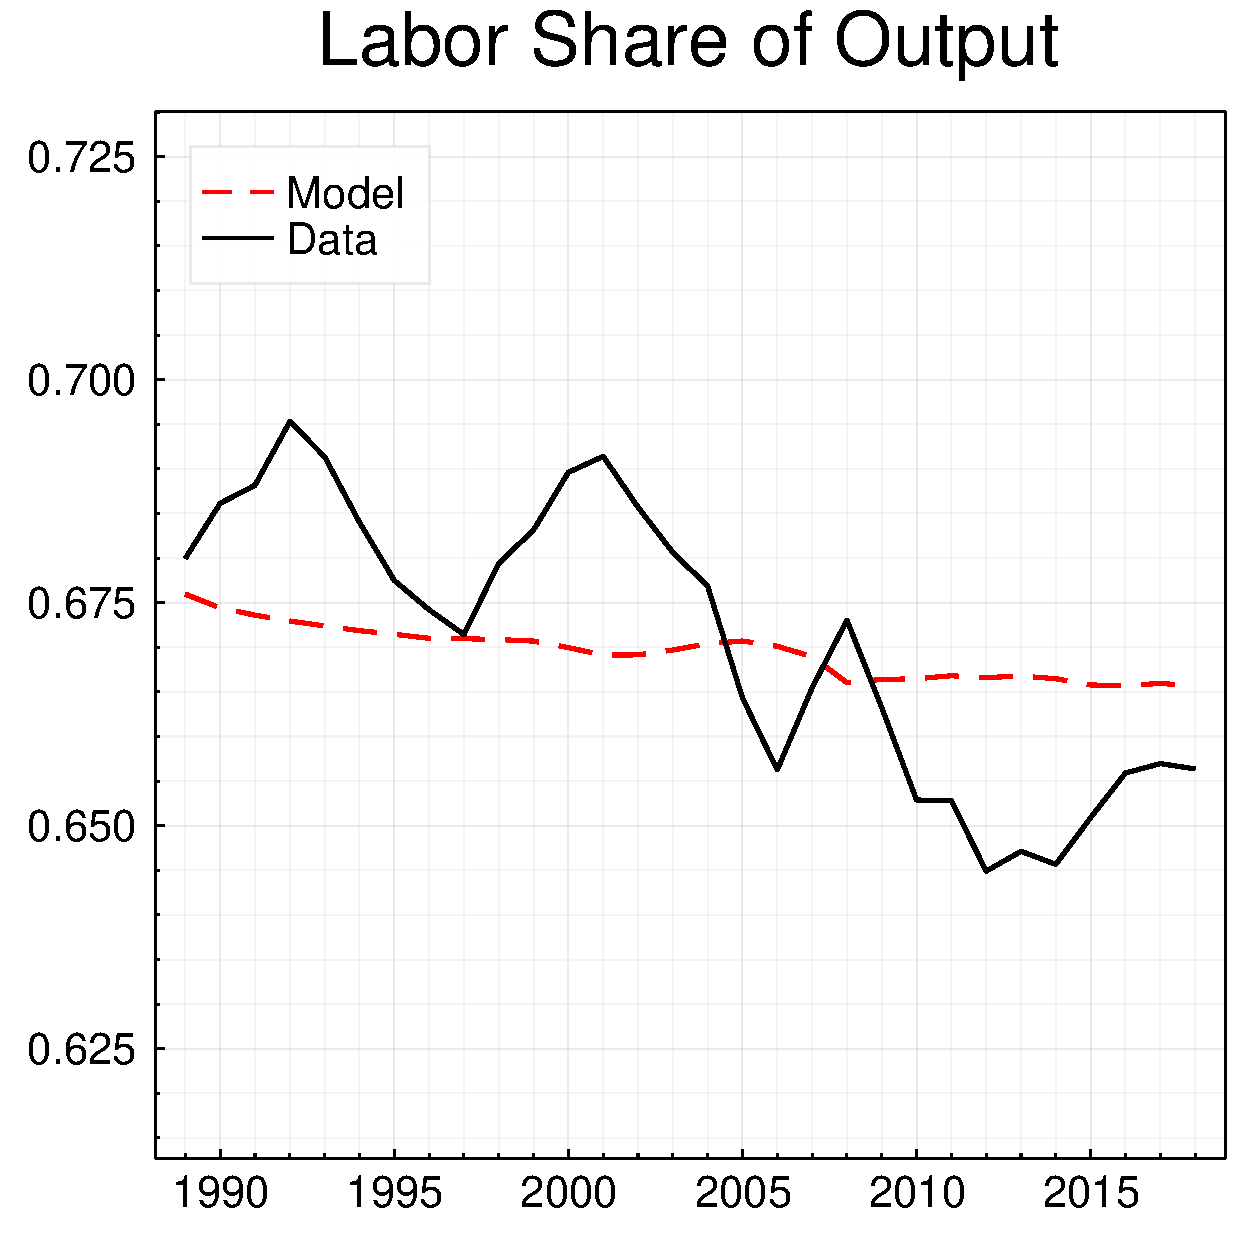
\includegraphics[width=0.3\textwidth]{../images/fig:updated_ind_estimation_ls_slides.pdf}
 \hfill
 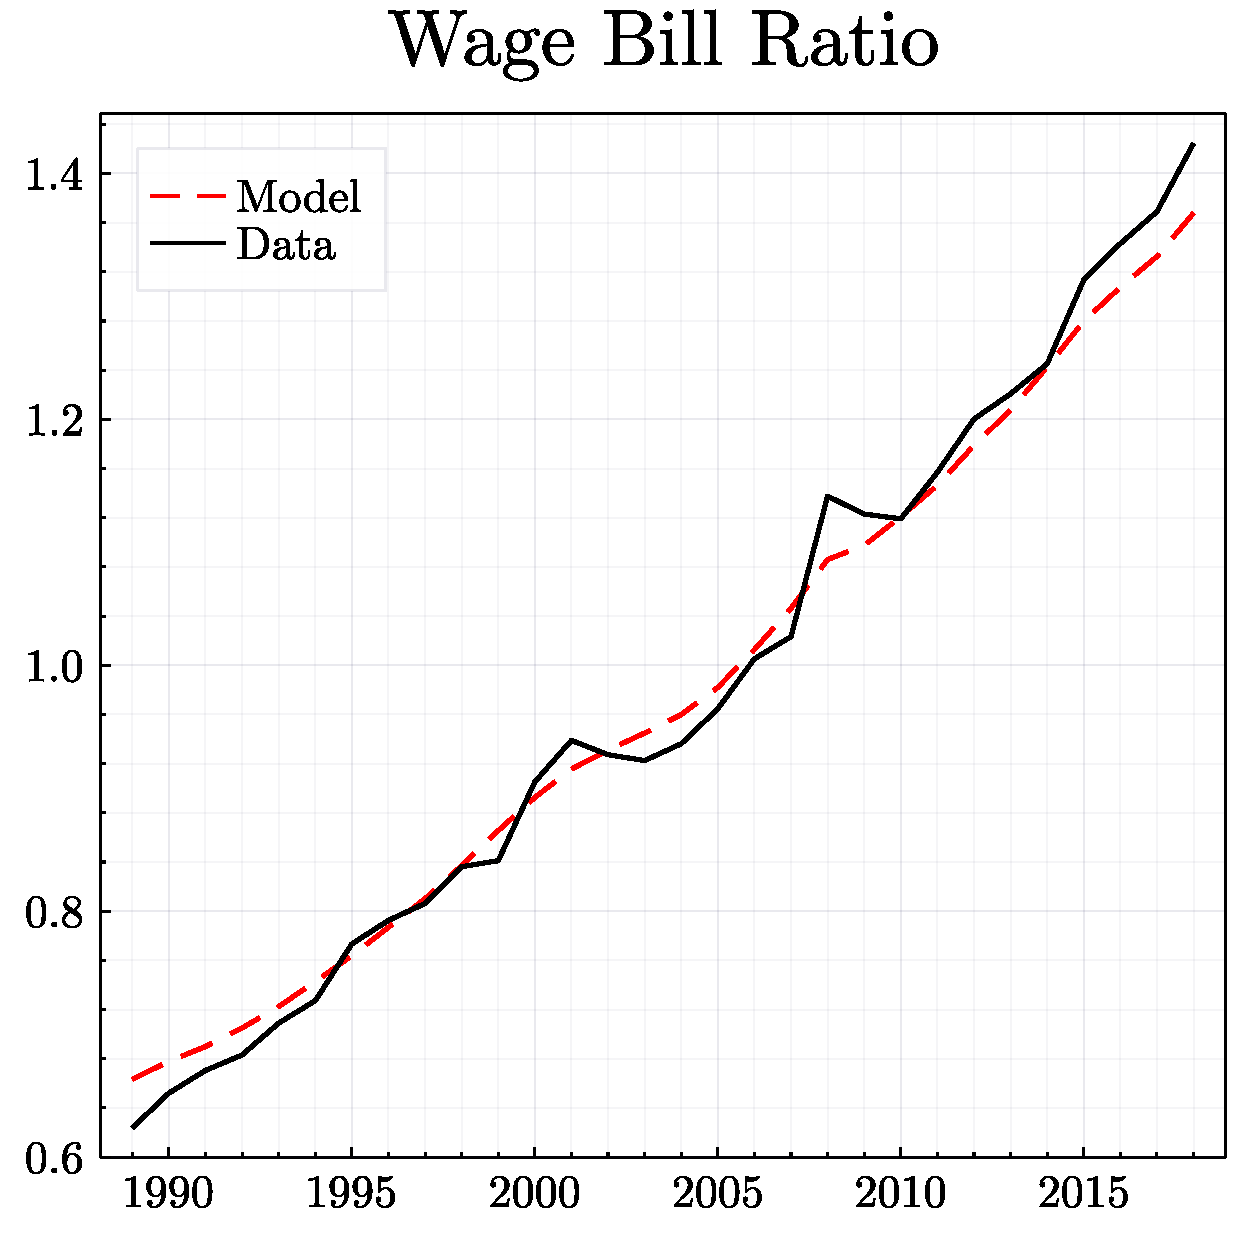
\includegraphics[width=0.3\textwidth]{../images/fig:updated_ind_estimation_wbr_slides.pdf}
 \hfill
 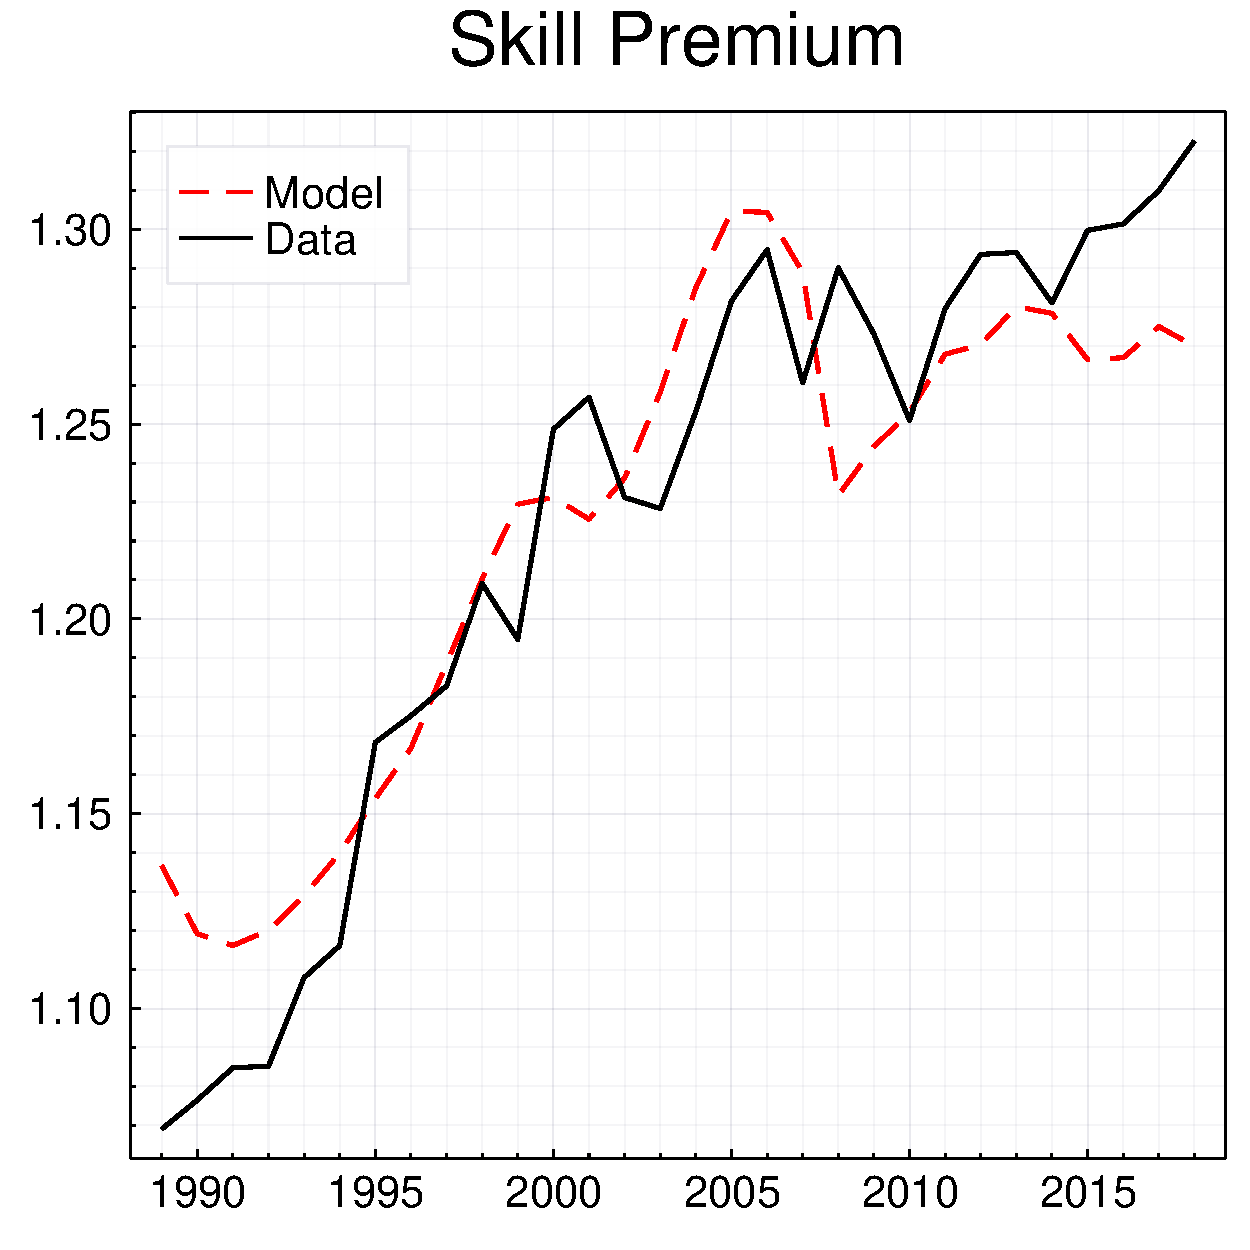
\includegraphics[width=0.3\textwidth]{../images/fig:updated_ind_estimation_sp_slides.pdf}
 \caption{\label{fig:korv_estimation_extended_industry} Fit for the $1988$ - $2018$ period with Updated Data.}
 \end{figure}
 }
\end{frame}

\begin{frame}
  \frametitle{Caveats}
  \begin{wideitemize}
    \item Convergence is highly sensitive to the initial conditions.
    \begin{wideitemize}
      \item Not a problem when estimating KORV.
      \item But when estimating the model for each industry, the initial conditions are not well defined.
    \end{wideitemize}
    \item Initially I tried to sweep the parameter space to find the best initial conditions, I tried a 10 values for each parameter (total of $700$ points), it took me more than a day to run the code.
    \item I settled on the trying 10 initial conditions.
  \end{wideitemize}
\end{frame}



\subsection{Industry Level Results}
\begin{frame}
 \frametitle{Industry Level Results}
 \begin{table}[h]
 \begin{center}
 \begin{tabular}{rrrrr}
  \hline\hline
    & \textbf{Updated Data} & \textbf{Industry Level}  & \textbf{Industry Level}  \\
    & \texttt{$1988$ - $2018$} & \texttt{(mean)} & \texttt{(std)} \\\hline
  $\alpha$ & 0.08 &  0.241 &  0.206 \\
  $\sigma$ & 0.313 &  0.483 &  0.710\\
  $\rho$ & -0.154 & -0.289 &  0.816\\
  $\eta_\omega$& 0.043 &  0.131 &  0.195\\\hline\hline
\end{tabular}
\end{center}
\caption{\label{tab:estimation_ind} Industry Level Estimates.}
\end{table}

\end{frame}

\begin{frame}
  \frametitle{Industry Level Results}
  \begin{wideitemize}
    \item On averegage the Capital-skill complementarity hypothesis $(\sigma > \rho)$ is holds at the industry level.
    \item Specifically, the hypothesis holds for for $44$ of $56$ ($78.8\%$) industries.
  \end{wideitemize}
 \end{frame}

\begin{frame}
  \frametitle{Future Work}

  \begin{wideitemize}
    
    
    \item Improve the estimation using an altertive methodology, e.g. 
    \begin{wideitemize}
      \item \textcolor{blue}{Polgreen, and Silos(2008)} discuss the sentitivity of KORV to variations in the data and propose a methodology to estimate the parameters that avoid the instabilities that can arise in maximizing a multidimensional function numerically
    \end{wideitemize}
      
    \item Incorporate alternative sources of data. Specifically, Quarterly Workforce Indicators (QWI) published as part of the Longitudinal Employer-Household Dynamics. This will allow me to avoid having to segment the CPS data to estimate the labor input and wage series at the industry level. 
  \end{wideitemize}

\end{frame}

% \section{Data}
% \begin{frame}[label=data]{Data}
% \centering
% \begin{wideitemize}
% \item A crucial step to take this model to data is to extend the original KORV data to the present.
% \item I follow the procedure by \cite{ohanian2021revisiting}.
% \item Capital stock series (both equipment and structures) are constructed from investment series from NIPA.
% \hyperlink{capital_data}{\beamergotobutton{Capital Data}}
% \item Labor data (wages and labor input of skilled and unskilled workers) is constructed from the ASEC of the CPS \hyperlink{labor_data}{\beamergotobutton{Labor Data}}
% \item Both capital and labor series can be also constructed at the industry level, which will allow us to estimate the model for each industry (2 or 3 NAICS digits).
% \end{wideitemize}
% \end{frame}

% \begin{transitionframe}
% \begin{center}
% { \Huge \textcolor{black}{Simulations}}
% \end{center}
% \end{transitionframe}

% \section{Simulation}


% \begin{frame}[label=sim_result]{Simulation Results}
% \begin{wideitemize}
 
% % \only<1-4>{
% \item \hyperlink{skil_prem<2>}{\beamergotobutton{Relative Quantity Effect}} $\sigma = 0.436 \quad \implies \quad \sigma^L > 1$
% % \only<2-4>{
% % \begin{center}
% % \includegraphics[width=.7\textwidth]{document/figures/quantity_effect.pdf}
% % \end{center}
% % \item \hyperlink{skil_prem<4>}{\beamergotobutton{Capital-Skill Complementarity Effect}} $\rho = -0.517 \quad \implies \quad \sigma > \rho \quad \implies \quad \sigma_L > \sigma_H$
% % % \only<4>{
% % \begin{center}
% % \includegraphics[width=.7\textwidth]{document/figures/cap_skill_complementarity.pdf}
% % \end{center}
% % }
% % }
 
% \end{wideitemize}
% \end{frame}

% \begin{frame}[sim_result]{Simulation Results\hyperlink{sim_korv_data}{\beamergotobutton{KORV Data}}}
% % \begin{center}
% % % \caption{Simulated Skill Premium from the Model}
% % \includegraphics[width=.65\textwidth]{document/figures/sim_skill_premium.pdf}
% % \end{center}
% \end{frame}


% \section{Future Work}
% \begin{frame}{Future Work}
% \begin{wideitemize}
% \item Estimate the model at the industry level. 
% \item Analyze how much variation in skill premium at the industry level is due to differences in estimated parameters.
% \item Try to implement a mechanism that links labor force composition, skill premium, and skill-biased technology from \textbf{KORV}.
% \end{wideitemize}
% \end{frame}
\section*{References}
\begin{frame}{References}
  \begin{itemize}
    \item Song, Jae, David J. Price, Fatih Guvenen, Nicholas Bloom, and Till Von Wachter. "Firming up inequality." The Quarterly journal of economics 134, no. 1 (2019): 1-50.
    \item Krusell, Per, Lee E. Ohanian, José‐Víctor Ríos‐Rull, and Giovanni L. Violante. "Capital‐skill complementarity and inequality: A macroeconomic analysis." Econometrica 68, no. 5 (2000): 1029-1053.
    \item Haltiwanger, John C., Henry R. Hyatt, and James Spletzer. Industries, mega firms, and increasing inequality. No. w29920. National Bureau of Economic Research, 2022.
    \item  Ohanian, Lee E., Musa Orak, and Shihan Shen. Revisiting capital-skill complementarity, inequality, and labor share. No. w28747. National Bureau of Economic Research, 2021.
    \item Acemoglu, Daron, and Pascual Restrepo. "Unpacking skill bias: Automation and new tasks." In aea Papers and Proceedings, vol. 110, pp. 356-61. 2020.
    \item Polgreen, Linnea, and Pedro Silos. "Capital–skill complementarity and inequality: A sensitivity analysis." Review of Economic Dynamics 11, no. 2 (2008): 302-313.
  \end{itemize}
 % \bibliographystyle{plainnat}
 % \bibliography{/Users/mitchv34/Work/industry_skill_premium/documents/manuscript/references.bib}
\end{frame}


% \appendix
% \subsection{Capital}
% \begin{frame}[label=capital_data]{Appendix: Capital Data \hyperlink{data}{\beamergotobutton{Back}}}
% \begin{wideitemize}
% \item To obtain annual series for both types of capital I use the Perpetual Inventory Method (PIM):
% $$k_{t+1}^{i} = (1 - \delta_{t}_{i})k_{t}^{i} + x_{t}^{i} \qquad i \in \{e,s\}$$
% \item Capital investment data for both equipment and structures dating from $1947$ are from the National Income and Product Accounts (NIPA).
% \item To iteratively generate the structures capital stock we need:
% \begin{itemize}
% \item The depreciation rates $\delta$ obtained, an initial value for $K_{1947}^i$, a deflator.
% \end{itemize}
% \end{wideitemize}
% \end{frame}

% \begin{frame}{Appendix: Capital Data}
% \begin{figure}[h]
% \caption{Updated Capital Structures and Equipment series (normalized to 1963=1)}
% \centering
% \includegraphics[width=.85\textwidth]{document/figures/capital_data_1.pdf}
% \end{figure}
% \end{frame}

% \begin{frame}{Appendix: Capital Data}\hyperlink{data}{\beamergotobutton{Back}}
% \begin{figure}[h]
% \caption{Ratios between purchases and prices (normalized to 1963=1)}
% \centering
% \includegraphics[width=.85\textwidth]{document/figures/capital_data_2.pdf}
% \end{figure}
% \end{frame}

% \subsection{Labor Input and Wages}

% \begin{frame}[label=labor_data1]{Appendix: Labor Input and Wages}
% \begin{wideitemize}
% \item To construct the wage and labor input series, I use the march supplement of the current population survey (CPS). \hyperlink{labor_data_appendix1}{\beamergotobutton{Sub Sample}}
% \item For each person, record: \hyperlink{labor_data_appendix2}{\beamergotobutton{Variables}}
% \begin{itemize} 
% \item their characteristics, employment statistics, income, and CPS personal supplement weights.
% \end{itemize}
% \item Workers are assigned to one of $264$ groups based on their characteristics. \hyperlink{labor_data_appendix3}{\beamergotobutton{Groups}}
% \item I calculated the average hours worked each year and the hourly wage for each group. \hyperlink{labor_data_appendix4}{\beamergotobutton{Group Averages}}
% \item Finally, I aggregate annual data on wages and hours distinguishing groups with a college degree ($H$) and non-college degrees ($L$) \hyperlink{labor_data_appendix5}{\beamergotobutton{Aggregation}}

% \end{wideitemize}
% \end{frame}
% \begin{frame}{Appendix: Labor Data}
% \begin{figure}[h]
% \caption{Wages and Labor Input (normalized to 1963=1)}
% \centering
% \includegraphics[width=1\textwidth]{document/figures/labor_data.pdf}
% \end{figure}
% \end{frame}


% \begin{frame}[label=labor_data_appendix1]{Appendix: CPS Sub-sample \hyperlink{labor_data1}{\beamergotobutton{Back}}}
% I include all observations excluding agents: 
% \begin{itemize}
% \item younger than $16$ or older than $70$.
% \item unpaid family workers.
% \item those working in the military.
% \item those who report working less than $40$ weeks a year and/or $35$ hours a week.
% \item individuals with allocated income.
% \item those with hourly wages below half of the minimum federal wage rate.
% \item those whose weekly pay was less than $\$62$ in $1980$ dollars (equivalent to $\$(2.022 \times 62)$ in $1999$ dollars).
% \item those did not report their education level
% \item self-employed are excluded for wage sample but used when constructing labor input series.
% \end{itemize}
% \end{frame}
% \begin{frame}[label=labor_data_appendix2]{Appendix: Variables\hyperlink{labor_data1}{\beamergotobutton{Back}}}
 
% \begin{wideitemize}
% \item their characteristics:
% \begin{itemize}
% \item age, sex, race 
% \end{itemize}
% \item employment statistics: 
% \begin{itemize}
% \item employment status (\texttt{empstat}).
% \item class of worker (\texttt{classwly}). 
% \item weeks worked last year (\texttt{wkswork1} and \texttt{wkswork2}).
% \item usual hours worked per week last year (\texttt{uhrsworkly} and hours work last week \texttt{ahrsworkt}. 
% \end{itemize}
% \item income:
% \begin{itemize}
% \item total wage and salary income \texttt{incwage}.
% \end{itemize}
% \item CPS personal supplement weights: \texttt{asecwt}.
% \end{wideitemize}
% \end{frame}
% \begin{frame}[label=labor_data_appendix3]{Appendix: Groups \hyperlink{labor_data1}{\beamergotobutton{Back}}}
 
% To homogenize the data I create the following groups based on individual characteristics:
% \begin{itemize}
% \item Age is divided into 11 five-year groups:
% \begin{itemize}
% \item $16-20 \ldots 66-70$. 
% \end{itemize}
% \item Race is divided into three: 
% \begin{itemize} 
% \item {white}, {black}, {others}
% \end{itemize}
% \item sex is divided into:
% \begin{itemize}
% \item male and female
% \end{itemize}
% \item education is divided into four groups:
% \begin{itemize}
% \item {below high school}, {high school}, {
% some college} and {college graduates and beyond}
% \end{itemize}
% \end{itemize}
% \end{frame}

% \begin{frame}[label=labor_data_appendix4]{Appendix: Group Averages\hyperlink{labor_data1}{\beamergotobutton{Back}}}
% \begin{wideitemize}
% \item For every individual I create the following variables:
% \begin{itemize}
% \item $\ell_{i,t}$ the hours worked by individual $i$ in year $t$, is the product of hours worked per week times weeks worked that year.
% \item $w_{i,t}$ the hourly wage of individual $i$ in year $t$, obtained by dividing yearly wage income by hours worked in year $t$.
% \end{itemize}
% \item Let $\mathcal{G}$ be the collection of all groups \item $\mu_{g,t} = \sum_{i\in g} \mu_{i,t}$ is the sum of CPS weight of the group.
% \item Average hours worked for each group $g\in\mathcal{G}$: 
% $$\ell_{g, t-1} = \frac{\sum_{i\in g}\ell_{i,t-1} \mu_{i,t}}{\mu_{g, t}} \quad \text{and} \quad
% w_{g, t-1} = \frac{\sum_{i\in g}w_{i,t-1} \mu_{i,t}}{\mu_{g, t}}$$
% \end{wideitemize}
% \end{frame}

% \begin{frame}[label=labor_data_appendix5]{Appendix: Aggregation \hyperlink{labor_data1}{\beamergotobutton{Back}}}
% \item Partition the set $\mathcal{G}$ in two subsets $(\mathcal{H}, \mathcal{L})$ based on education (college graduates and non-college graduates). 
 
% \item Total labor input:
% $$L^H_{t-1} = \sum_{g \in\mathcal{H}} \ell_{g, t-1} \mu_{g,t} \quad \text{and} \quad L^L_{t-1} = \sum_{g \in\mathcal{L}} \ell_{g, t-1} \mu_{g,t}$$
 
% \item and wages for each skill level:
 
% $$W^H_{t-1} = \frac{\sum_{g \in \mathcal{H}} w_{g, t-1} \elll_{g, t-1} \mu_{g,t}}{L^H_{t-1}}\quad \text{and} \quad W^L_{t-1} = \frac{\sum_{g \in \mathcal{L}} w_{g, t-1} \ell_{g, t-1} \mu_{g,t}}{L^L_{t-1}}$$ 
% % 
% \end{frame}

% \begin{frame}[label=sim_korv_data]{Simulation using KORV Data and Parameters\hyperlink{sim_result}{\beamergotobutton{Back}}}
% \begin{center}
% % \caption{Simulated Skill Premium from the Model}
% \includegraphics[width=.65\textwidth]{document/figures/sim_skill_premium_korv.pdf}
% \end{center}
% \end{frame}

\end{document}